\chapter{Evaluation and Results}
\label{Chapter5}

Having developed our distance-based approach for constrained procedural terrain generation and the Interactive Genetic Algorithm for parameter optimisation, we now finally turn to evaluating the effectiveness of our system. This chapter presents a comprehensive assessment of our approach through visual quality analysis, performance measurements, and comparative analysis. 

\section{Evaluation Methodology}

Our evaluation methodology combines visual assessment with performance analysis to provide an understanding of the system's capabilities. We recognise that terrain quality is \textit{inherently subjective} and context-dependent, making pure quantitative metrics insufficient for capturing the nuanced aspects of ``natural'' terrain appearance. Therefore, the visual assessment is based on our subjective judgement, but we aim to be consistent and reasonable by using clear criteria as described in the following Section \ref{visual_crit}. 

\subsection{Visual Quality Assessment}
\label{visual_crit}

Defining what constitutes ``natural-looking'' terrain presents an interesting challenge in procedural generation. For our evaluation, we establish several visual criteria that guide our assessment:

\begin{itemize}
    \item \textbf{Smooth Transitions}: The terrain should exhibit seamless blending between fixed and procedurally generated areas, without visible boundaries or abrupt height changes that betray the constraint locations;
    
    \item \textbf{Geological Possibility}: Generated features should resemble formations that could exist in \textbf{nature}, avoiding mathematically perfect patterns or unrealistic configurations that immediately signal algorithmic generation;
    
    \item \textbf{Contextual Coherence}: The terrain must appear as though the fixed elements (roads, buildings, water bodies, etc.) were naturally placed within an existing landscape, rather than the landscape being artificially constructed around them. However, if the constraints are unnatural looking themselves, we cannot expect the overall terrain to look good, as we can not modify the predefined constraints, and can only do our best with the modifiable areas;
    
    \item \textbf{Feature Variety}: Natural terrain exhibits variation in both large-scale features (hills, valleys) and fine details (surface texture, erosion patterns). Our generated terrain should demonstrate similar multi-scale variety.
\end{itemize}

While we acknowledge the subjective nature of visual assessment, we aim to be reasonable and critical in our analysis of our own results. We will also compare the visual results of our solutions with previous solutions based on these criteria. 

\subsection{Performance Metrics}
\label{performance_metrics}

Instead of just evaluating visual quality, we also wanted our system to run quickly. Although the time complexity of algorithms has been discussed in previous chapter, we will also measure the actual time it takes to perform certain tasks related to using our system. All the performance evaluation focuses on practical usability within the Unity development environment. All tests were conducted on an Apple MacBook Air (2025) with Apple M4 chip and 16GB RAM, running Unity 6000.0.41f. While absolute timing values are hardware-dependent, the relative performance differences between operations and approaches remain informative. 
We decided against analysing the memory usage of our system, as our system did not have an objective to be memory efficient. Memory also does not tend to be a limiting factor for adoption of a procedural terrain generation system, and most systems related to this have similar memory usage.


\section{Test Scenarios and Case Studies}
\label{case_studies}

Our evaluation explores diverse constraint patterns that we created representing real-world use cases. Each test scenario challenges different aspects of the system, some testing how it handles connected constraints, other testing how it handles constraints with extreme height disparities. We aim to display and evaluate a variety of example case studies to show the versatility and results of our system, and we believe that the five test cases discussed in this section adequately demonstrate this. 

Since our system also allows great flexibility in the users' preference of taste, whether they desire a smooth terrain of rolling hills or a rough and eroded mountain range, the final terrain is ultimately influenced by their choices, regardless of whether they are interacting with it through the manual approach or IGA approach. We try to have a slightly different preference in our taste in each case study, depending on what we decide would look good for the specific input constraint. 

As our system can handle two approaches of generation (see section \ref{interaction_models}), we will show an example of a terrain generated using each approach: (1) the manual approach and (2) generated using the Interactive Genetic Algorithm. When evaluating the manual approach, we will not provide the details of the exact terrain operations and their respective parameters that were applied to achieve this resulting terrain. We omit this information for the sake of brevity and because this section is rather to show what is possible with our system, not the exact instructions to achieve a specific result for a given example. Note that this section focuses only on \textbf{visual quality assessment} according to the criteria established in Section \ref{visual_crit}, and \textbf{performance evaluation} will be discussed in Section \ref{performance_eval}. \footnote{For readers interested in hands-on experimentation, our Unity project (see User documentation) includes numerous pre-configured scenes with masks and terrain setups.  This allows immediate testing without the overhead of creating custom constraint configurations, lowering the barrier to exploring the system's capabilities.}

% Case Study 1
\subsection{Road/Path network constraint}

This case study aims to show our systems ability to deal with linear features at reasonably similar elevation levels, testing the system's ability to create natural landscape around roads, race tracks and paths. 
In our example, we will use the constraint combination as seen in Fig. \ref{fig:constraint_1}, with the mask texture seen on the left, and the respective predefined heights seen on the right. 

% \hfill

\begin{figure}[h]
    \centering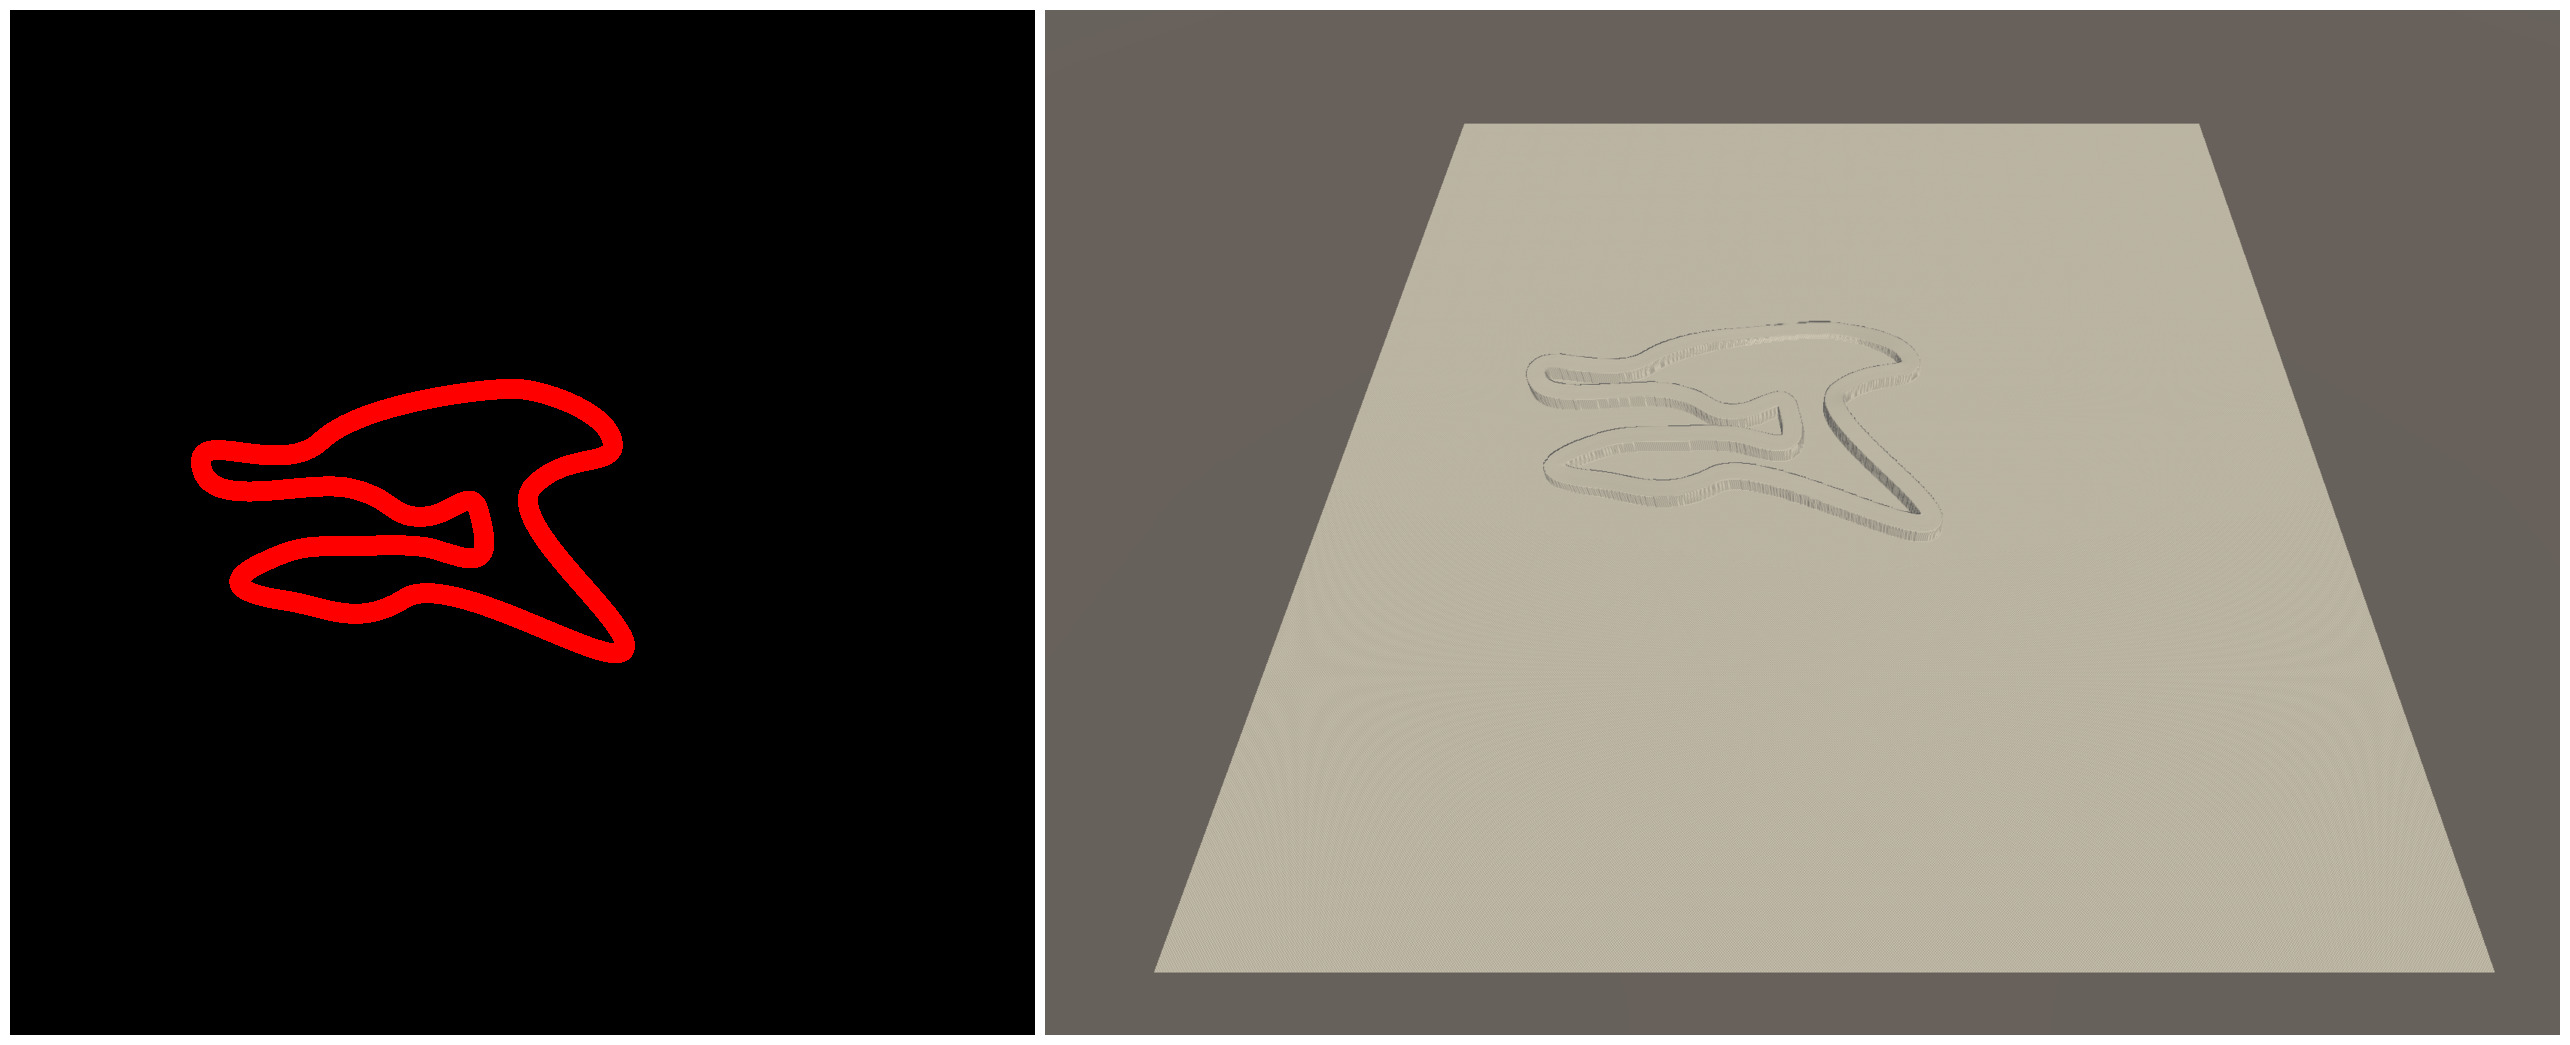
\includegraphics[width=0.65\linewidth]{img/evaluation/1/constraint_1.jpg}
    \caption{The input into our system. (Left) shows the mask texture provided. (Right) shows the set heights for the pixels mapped out by the mask texture.}
    \label{fig:constraint_1}
\end{figure}


% \hfill

\textbf{Manual Approach:} In Figure \ref{fig:manual_image_1}, we can see an example of a terrain generated using the manual interaction approach.

\begin{figure}[h]
    \centering
    \includegraphics[width=0.6\linewidth]{img/evaluation/1/manual_image_1.png}
    \caption{Resulting terrain of \ref{fig:constraint_1} generated using manually set terrain operations.}
    \label{fig:manual_image_1}
\end{figure}


% \hfill

% \hfill


\textbf{IGA Approach:} In Figure \ref{fig:iga_image_1}, we can see an example of a terrain generated using the IGA approach.

\begin{figure}[H]
    \centering
    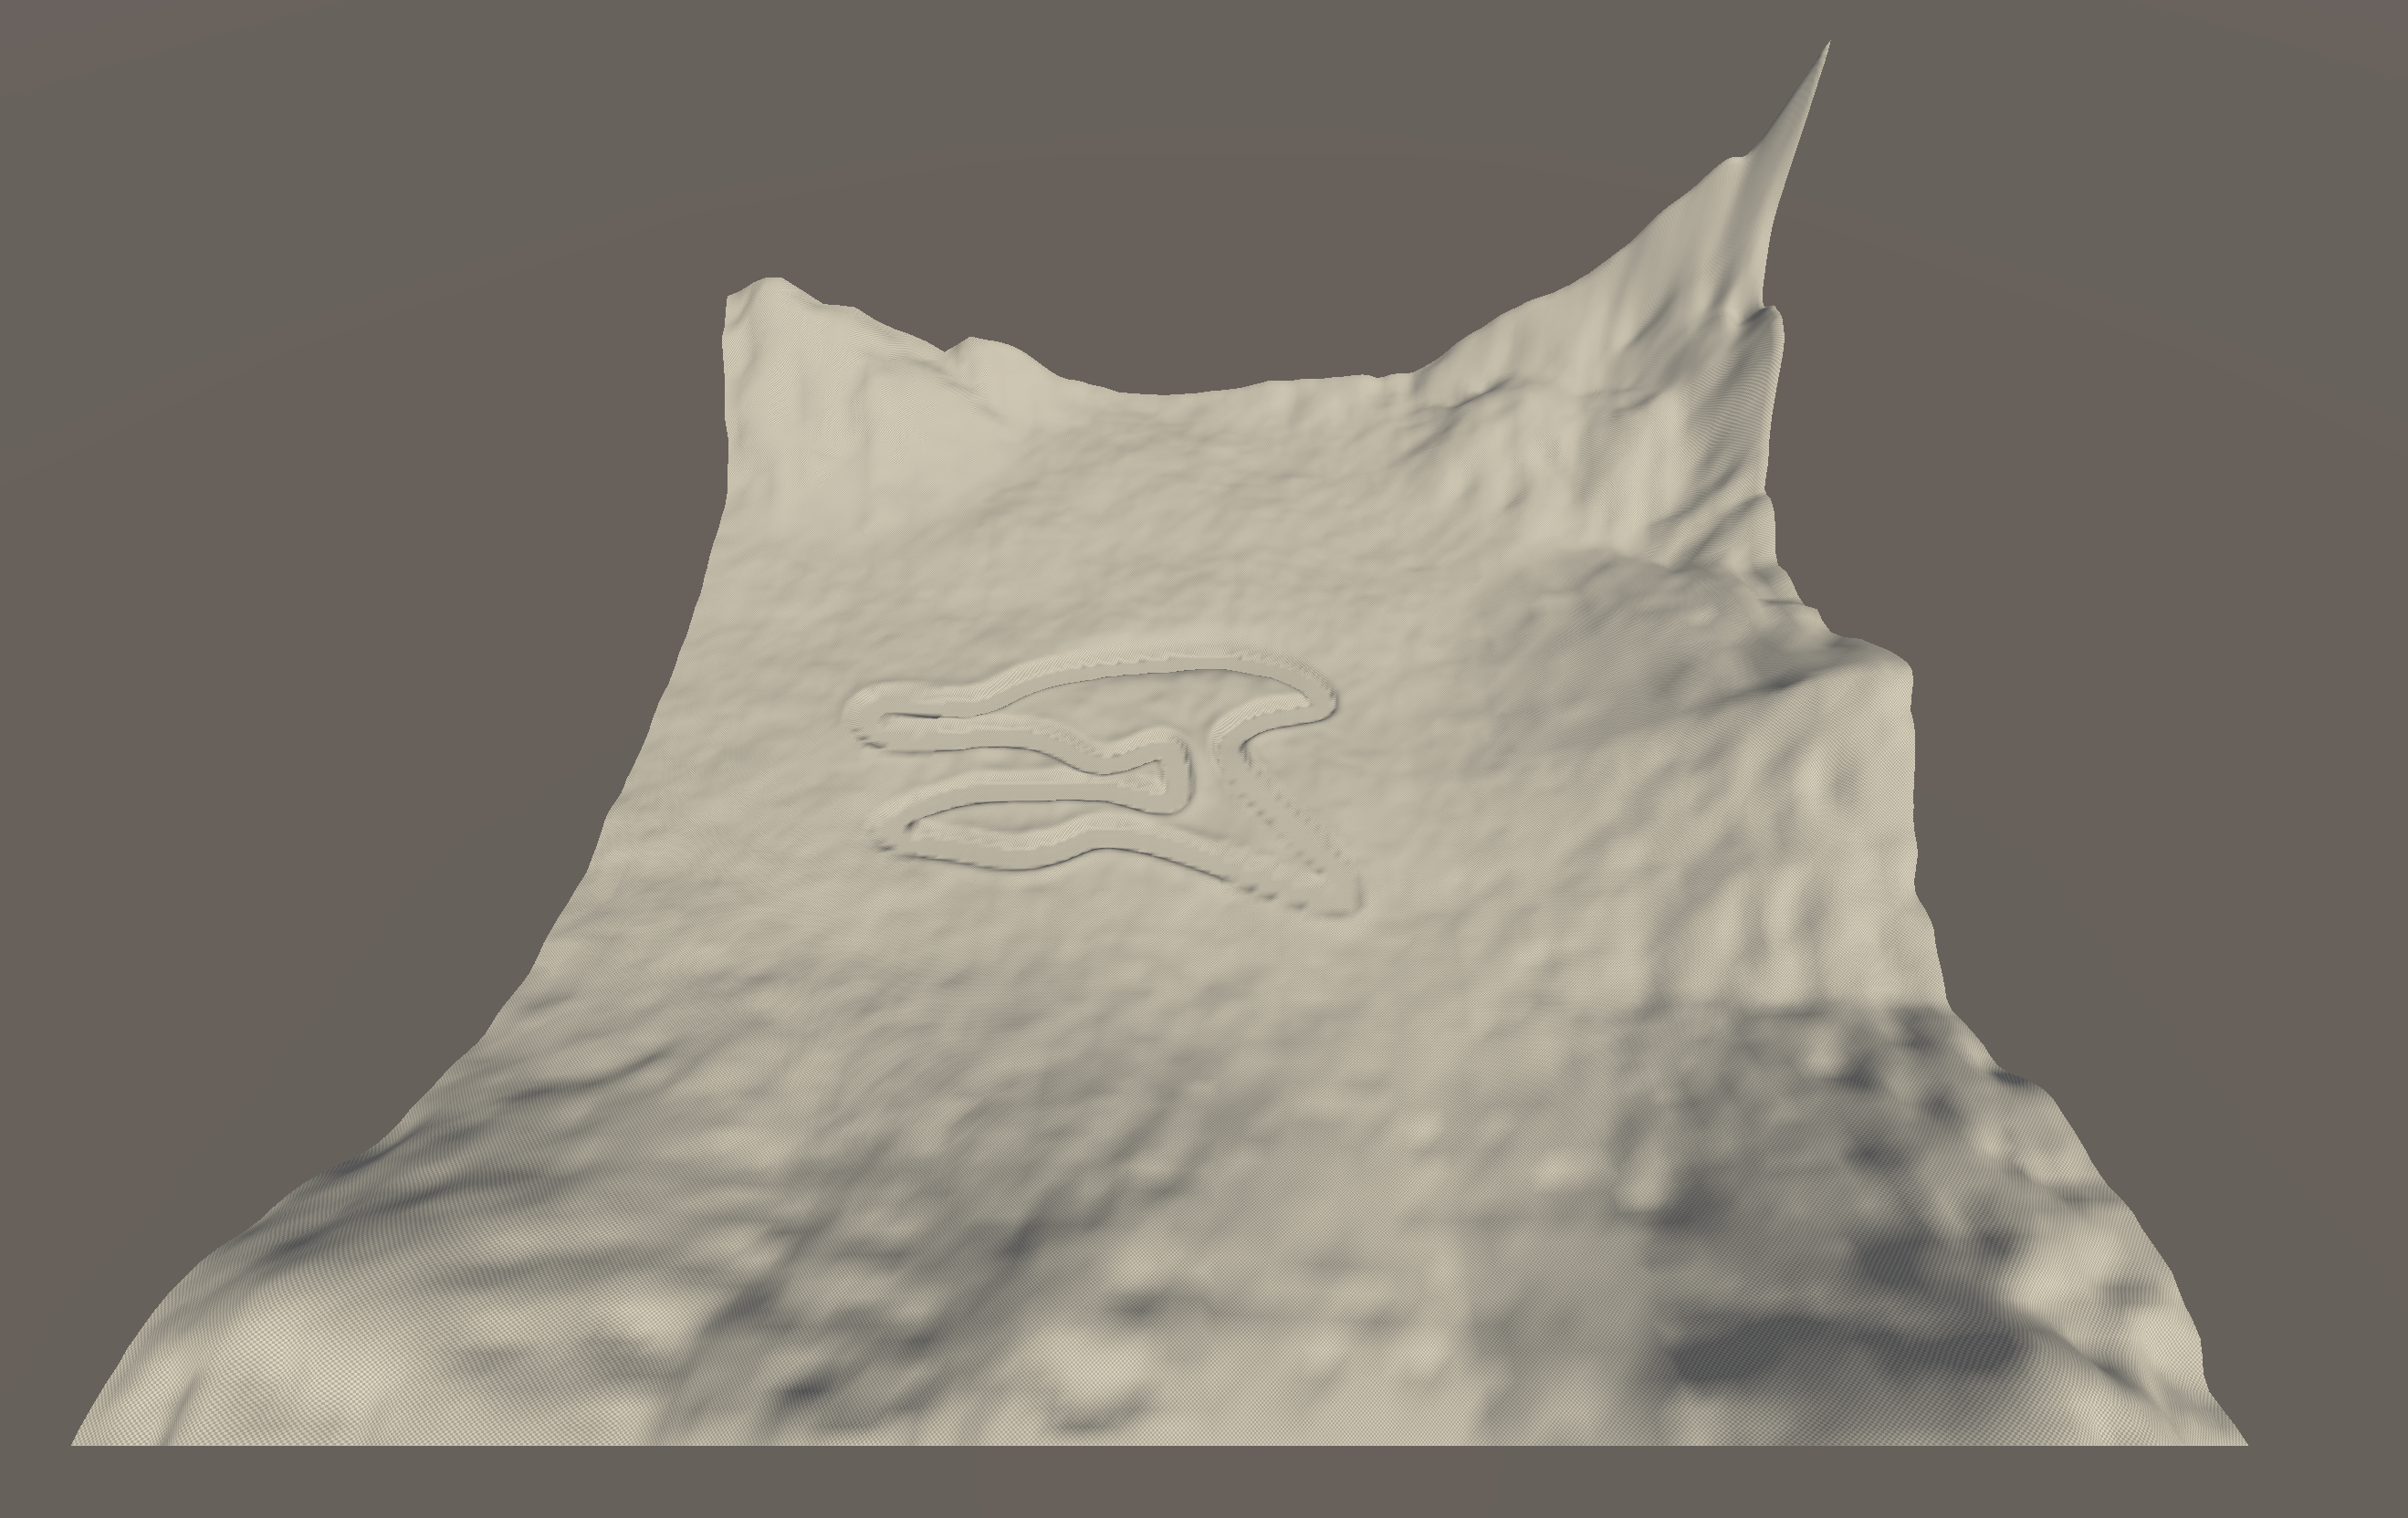
\includegraphics[width=0.6\linewidth]{img/evaluation/1/iga_image_1.png}
    \caption{Resulting terrain of \ref{fig:constraint_1} generated using the IGA evolution window.}
    \label{fig:iga_image_1}
\end{figure}


% Case Study 2
\subsection{Foundations constraint}
In this specific use case, it is important to note that our system has the objective to blend the surrounding terrain into the fixed areas, so we will not be testing or evaluating examples that would not normally have this in the real world (e.g. houses, trees or objects). This thesis focuses on only the procedural terrain generation of the heightmap, not on object placement.

However, if a developer is using our system, and they want to effectively place objects on top of the terrain in specific areas at given heights, we recommend they (1) draw this foundation, (2) generate the terrain, and (3) then place the objects on top of the terrain as they please. 

This way, the foundations on which the objects are placed will blend naturally into the surrounding terrain, and the objects they place will sit on top of these at the desired location and height.

Here we aim to show our system's ability to deal with disconnected foundation blocks placed around the terrain, each with a different uniform height. We will use the constraint combination as seen in Figure \ref{fig:constraint_2}: 

\begin{figure}[H]
    \centering
    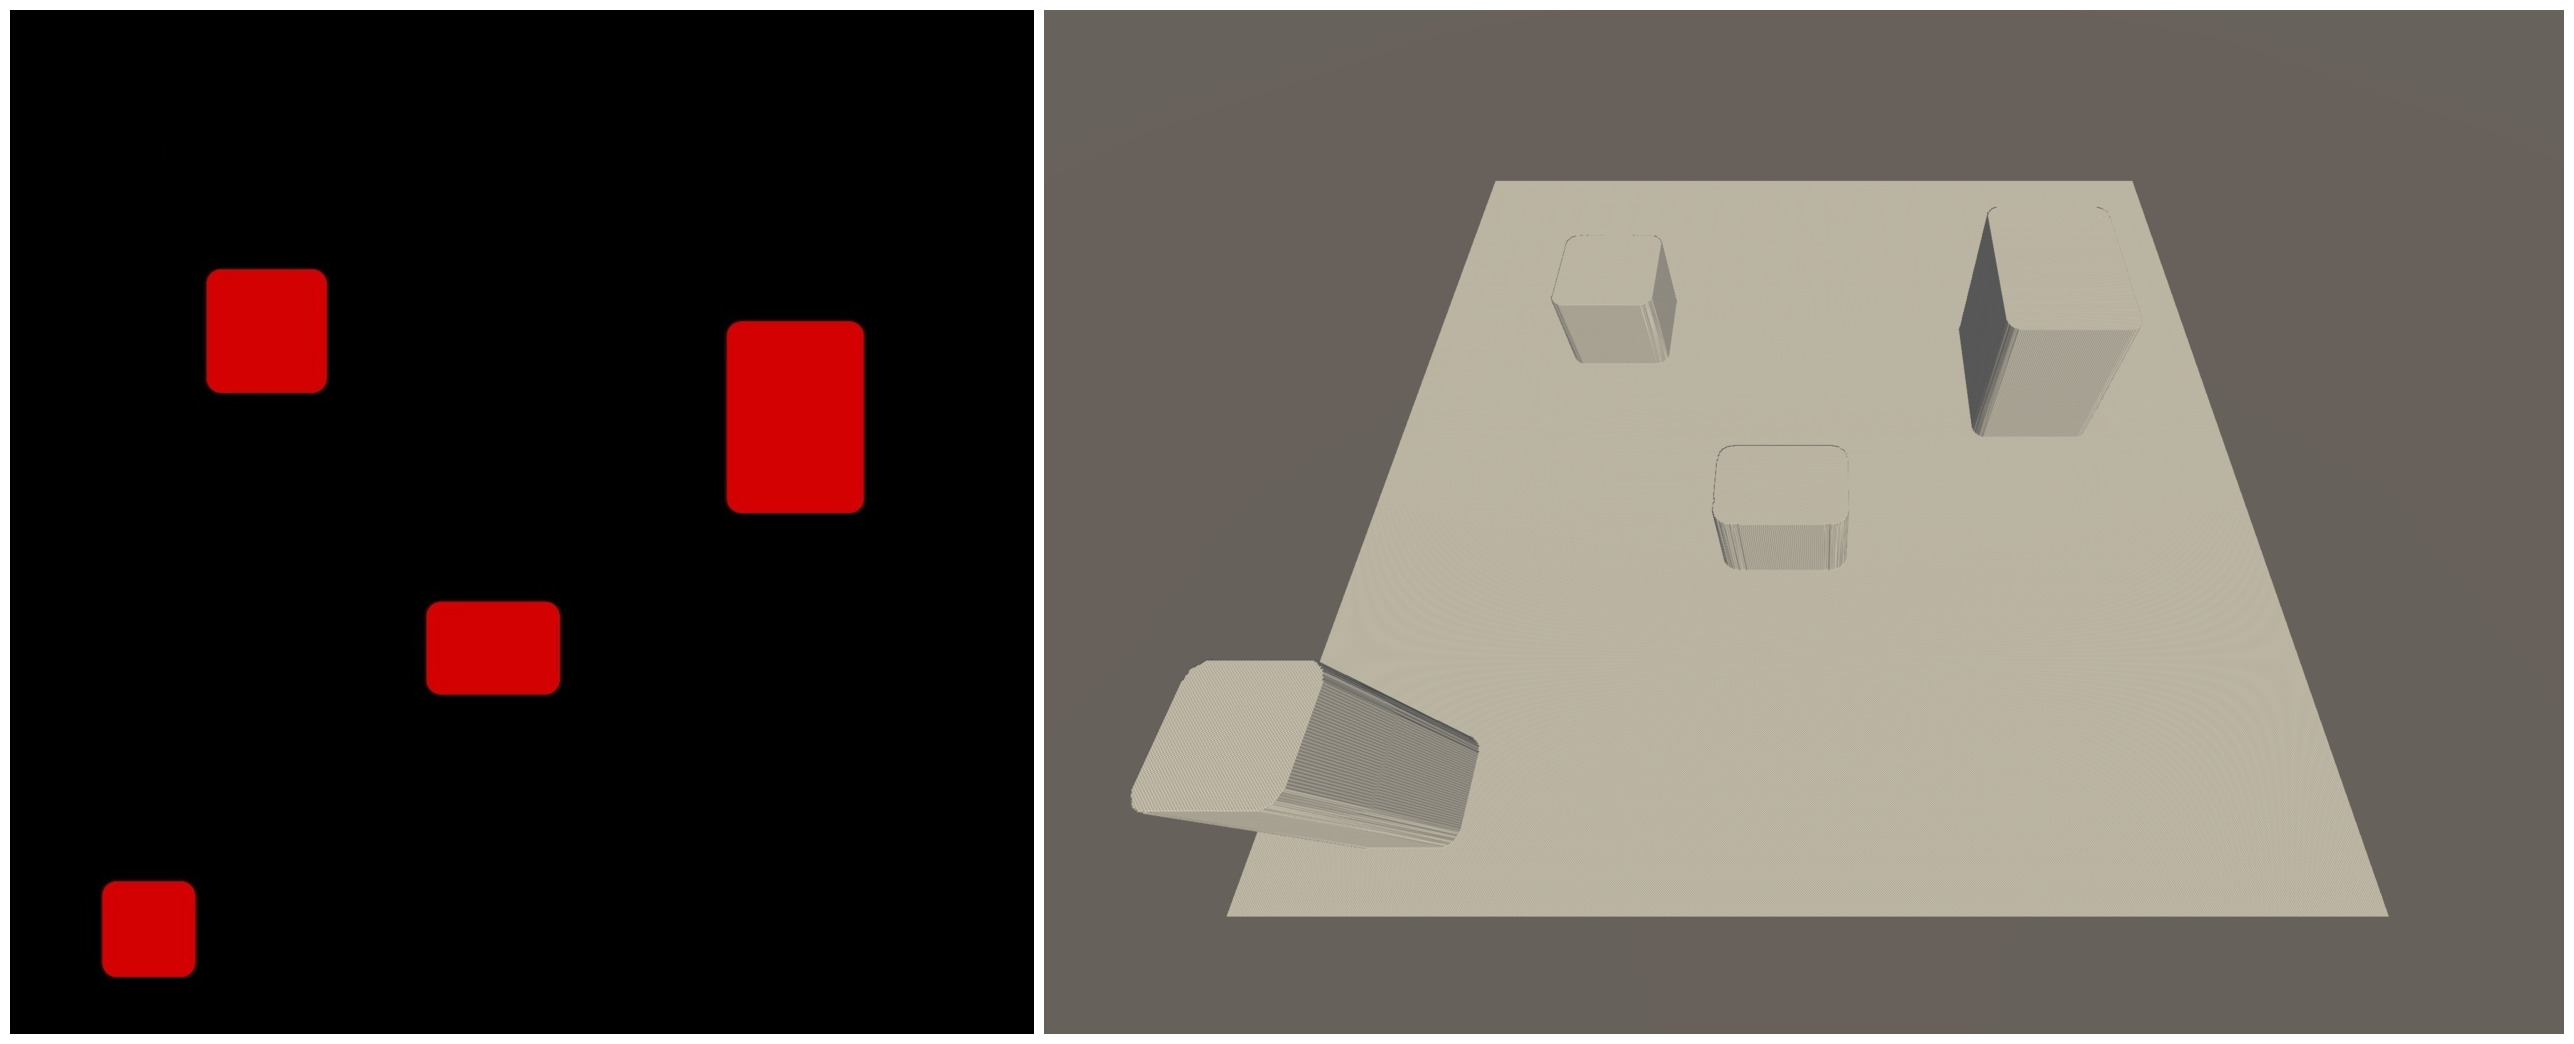
\includegraphics[width=0.7\linewidth]{img/evaluation/2/constraint_2.jpg}
    \caption{The input into our system. (Left) shows the mask texture provided. (Right) shows the set heights for the pixels mapped out by the mask texture.}
    \label{fig:constraint_2}
\end{figure}

\textbf{Manual Approach:} In Fig. \ref{fig:manual_image_2}, we can see an example of a terrain generated using the manual interaction approach.

\begin{figure}[H]
    \centering
    \includegraphics[width=0.7\linewidth]{img/evaluation/2/manual_image_2.png}
    \caption{Resulting terrain for \ref{fig:constraint_2} generated using manually set terrain operation.}
    \label{fig:manual_image_2}
\end{figure}

\textbf{IGA Approach:} In Fig. \ref{fig:iga_image_2}, we can see an example of a terrain generated using the IGA approach.

\begin{figure}[H]
    \centering
    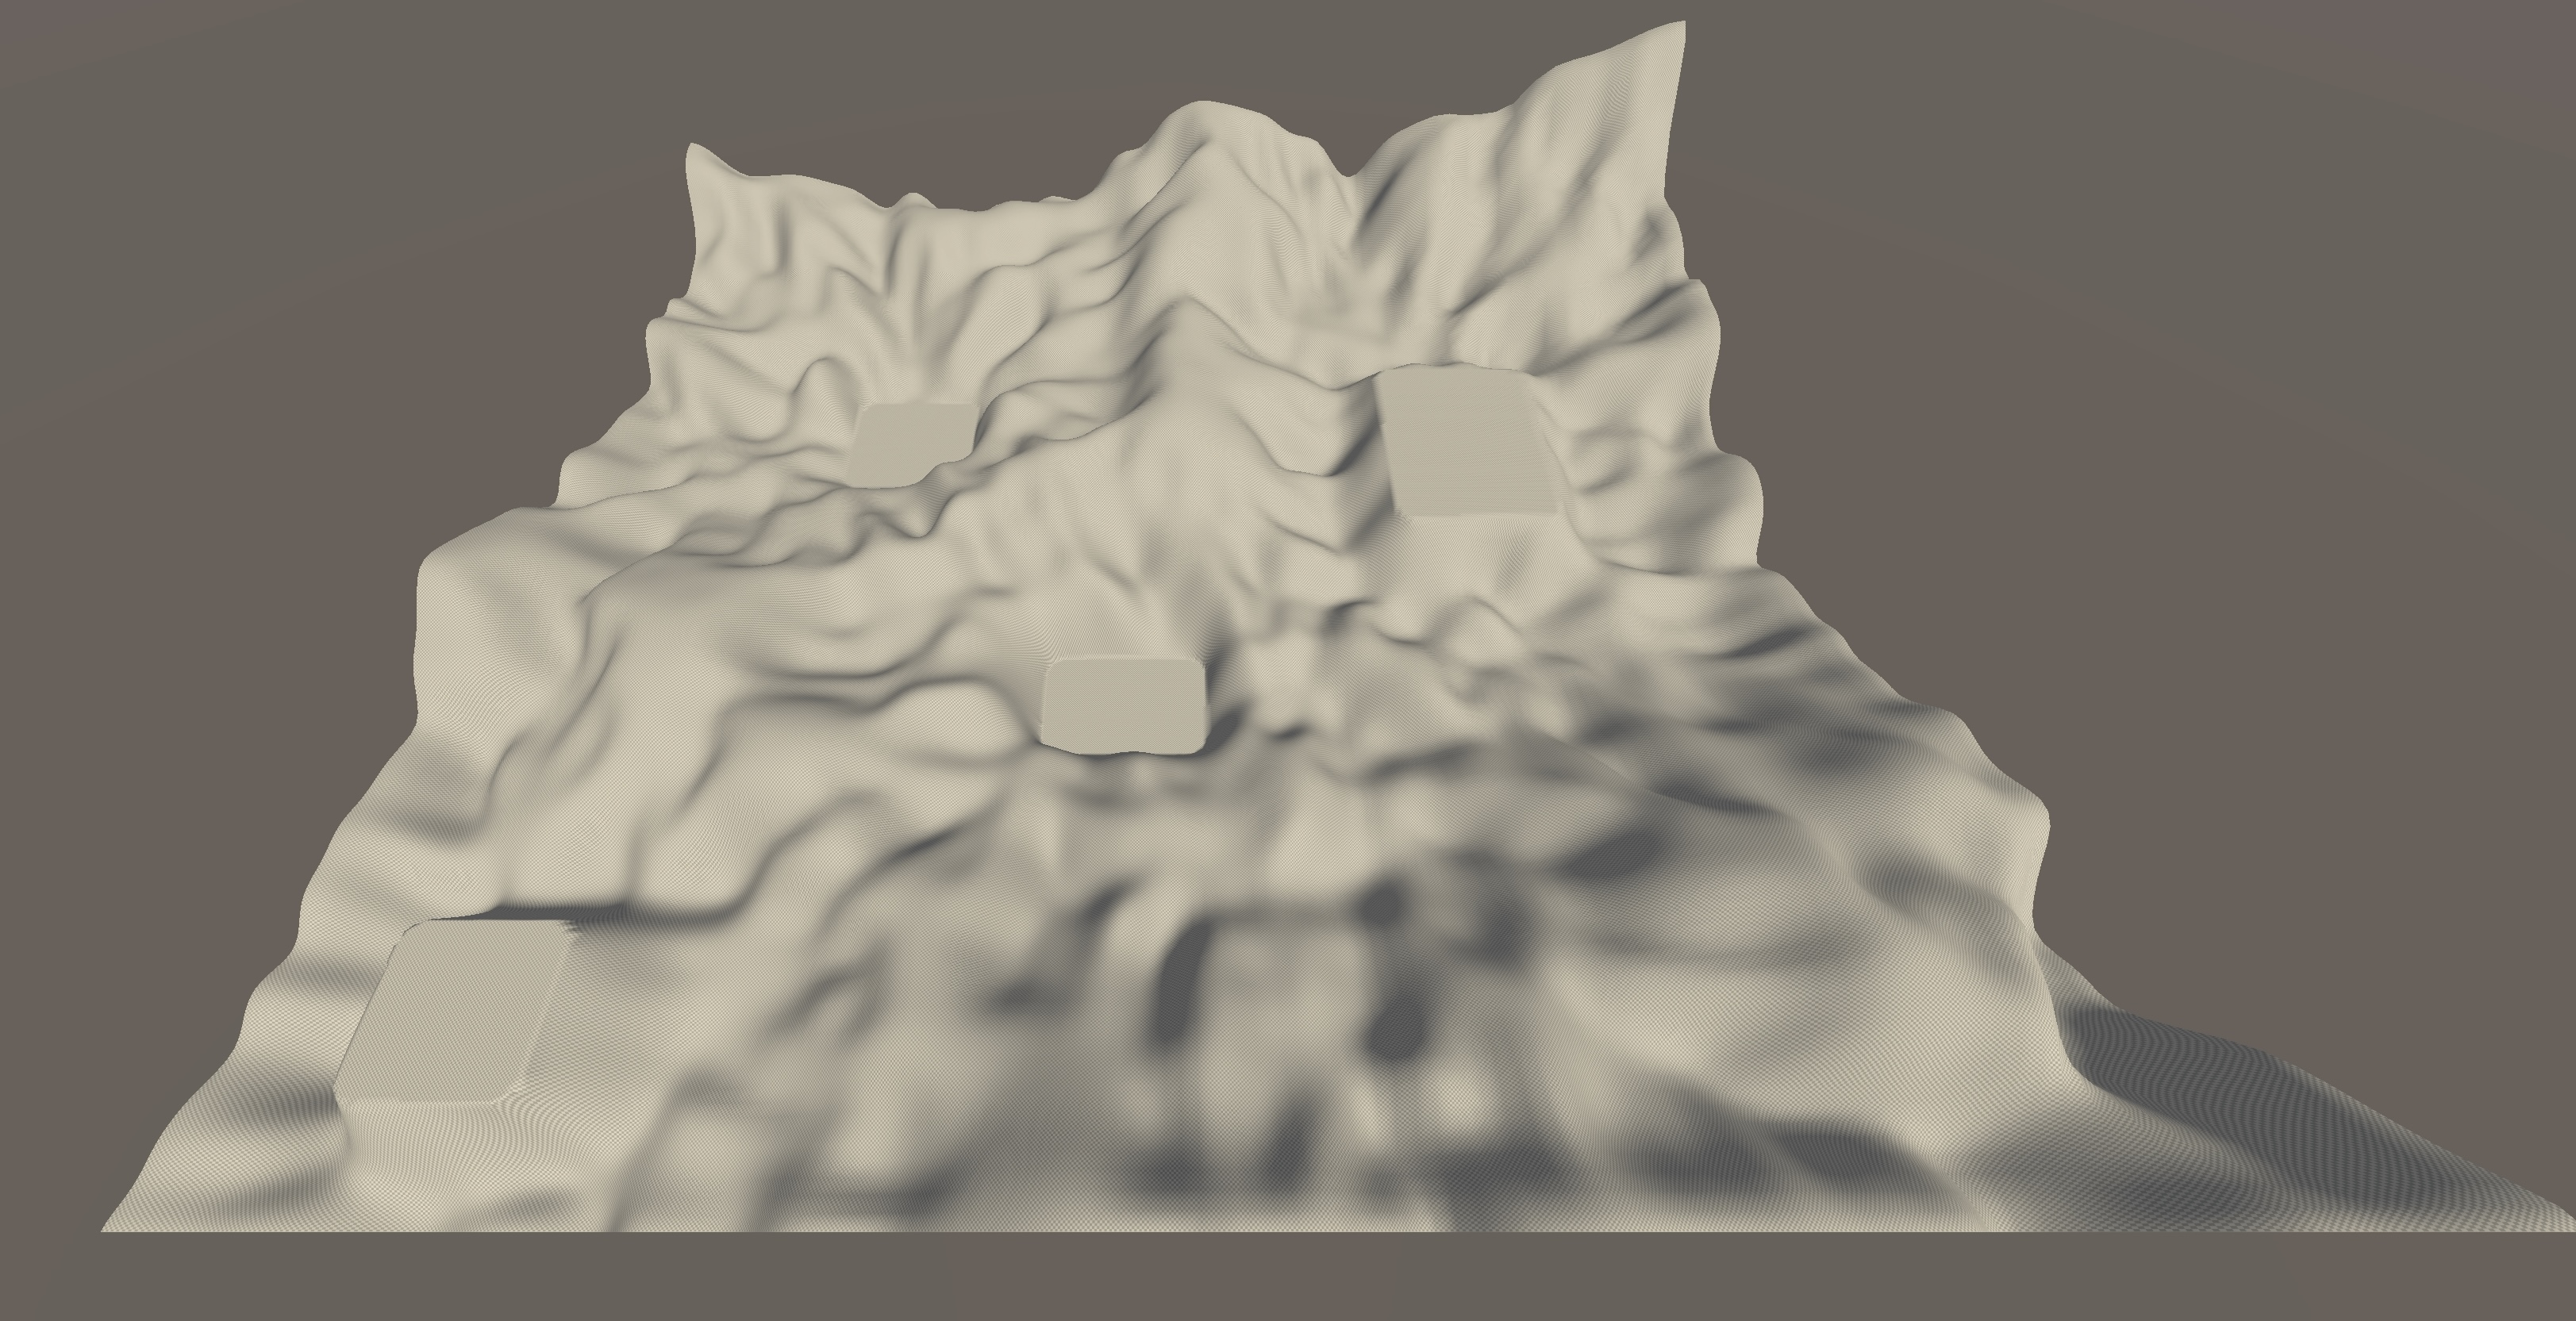
\includegraphics[width=0.6\linewidth]{img/evaluation/2/iga_image_2.jpg}
    \caption{Resulting terrain for \ref{fig:constraint_2} generated using the IGA evolution window.}
    \label{fig:iga_image_2}
\end{figure}

% Case Study 3
\subsection{River Network constraint}

This case study aims to show our system's ability to deal with constraints that could resemble a river network. A similar mask could also represent the ridge lines of a mountain range. The heights start high at the source of the river, and decrease as the river flows downhill.
In our example, we will use the constraint combination as seen in Fig. \ref{fig:constraint_3}, with the mask texture seen on the left, and the respective predefined heights seen on the right.

\begin{figure}[H]
    \centering
    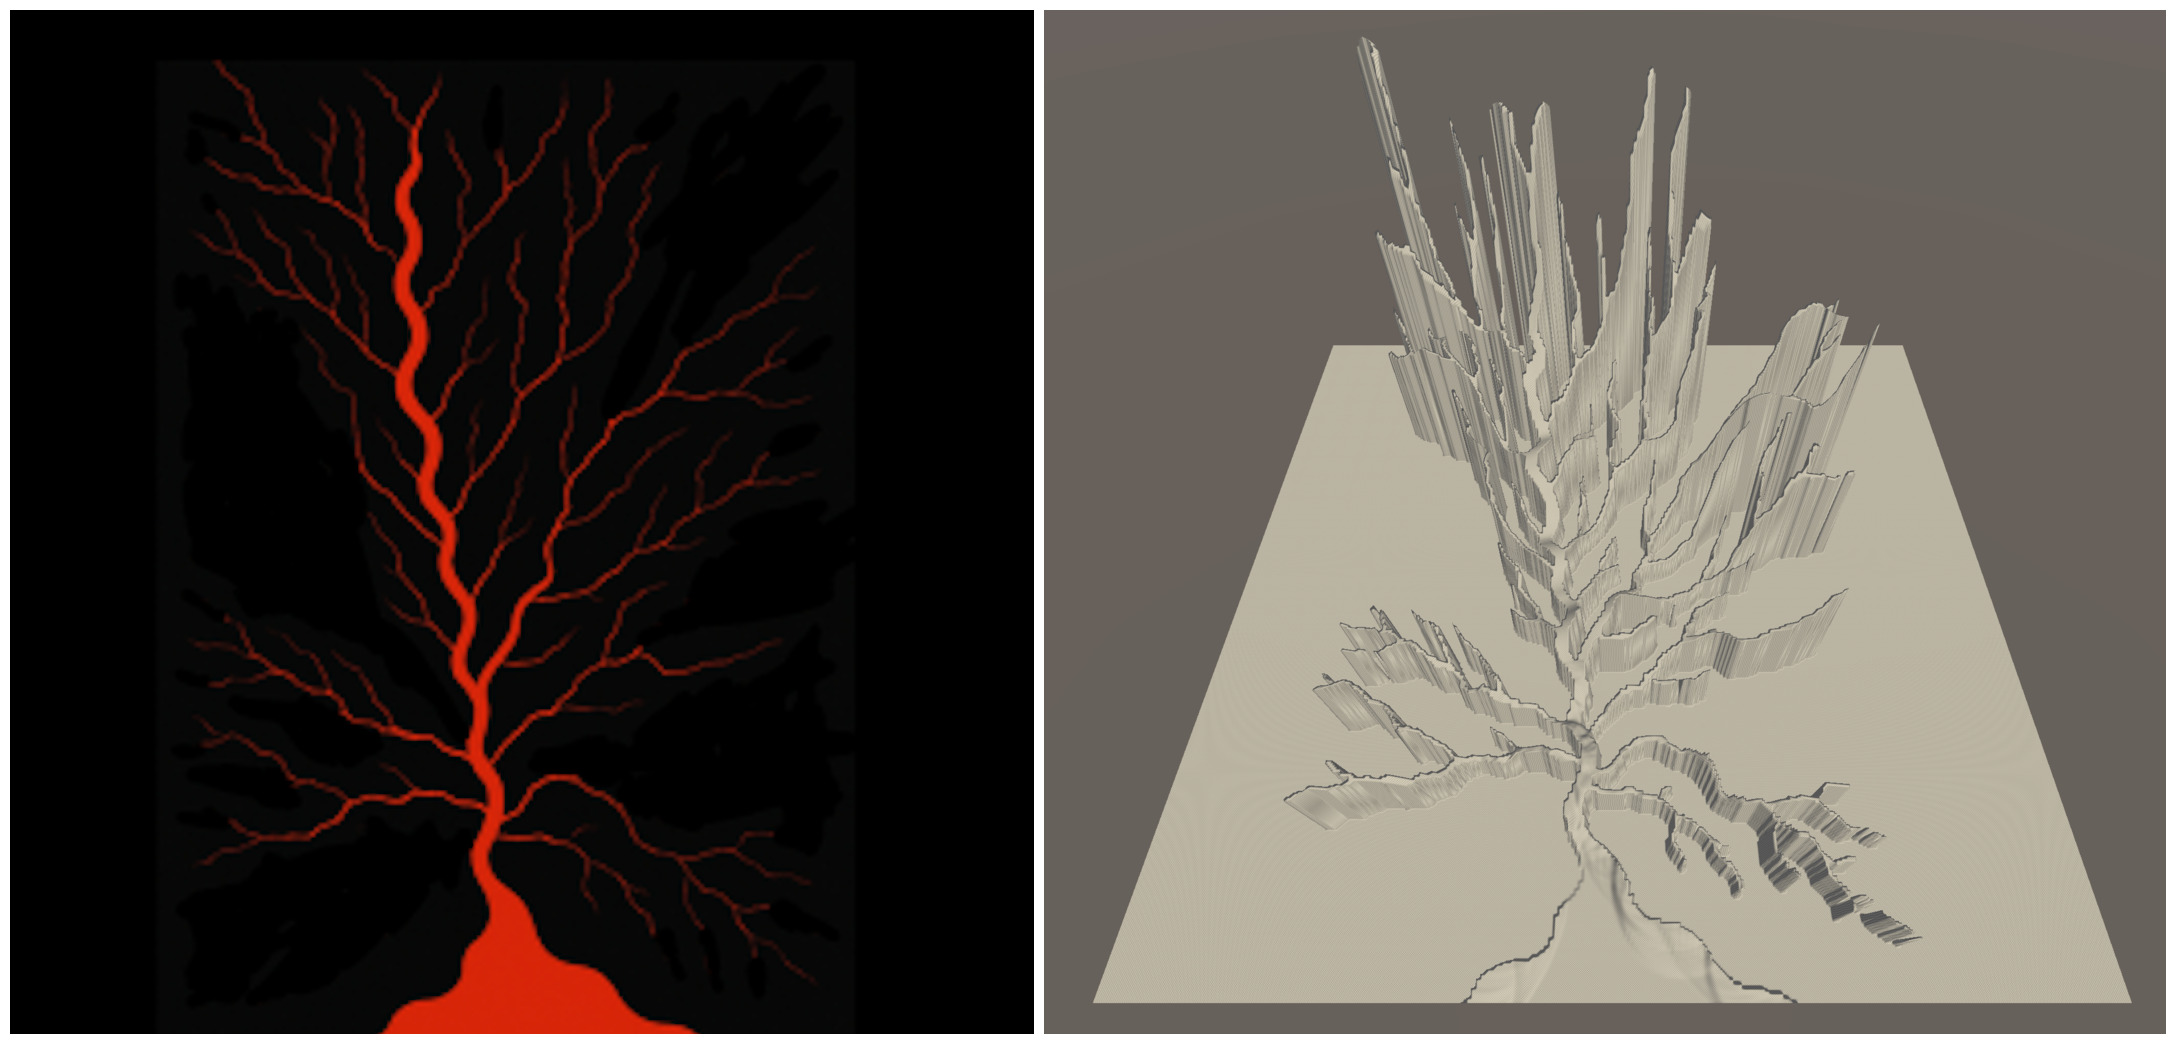
\includegraphics[width=0.6\linewidth]{img/evaluation/3/constraint_3.jpg}
    \caption{The input into our system. (Left) shows the mask texture provided. (Right) shows the set heights for the pixels mapped out by the mask texture.}
    \label{fig:constraint_3}
\end{figure}

\textbf{Manual Approach:} In Fig \ref{fig:manual_image_3}, we can see an example of a terrain generated using the manual interaction approach.

\begin{figure}[H]
    \centering
    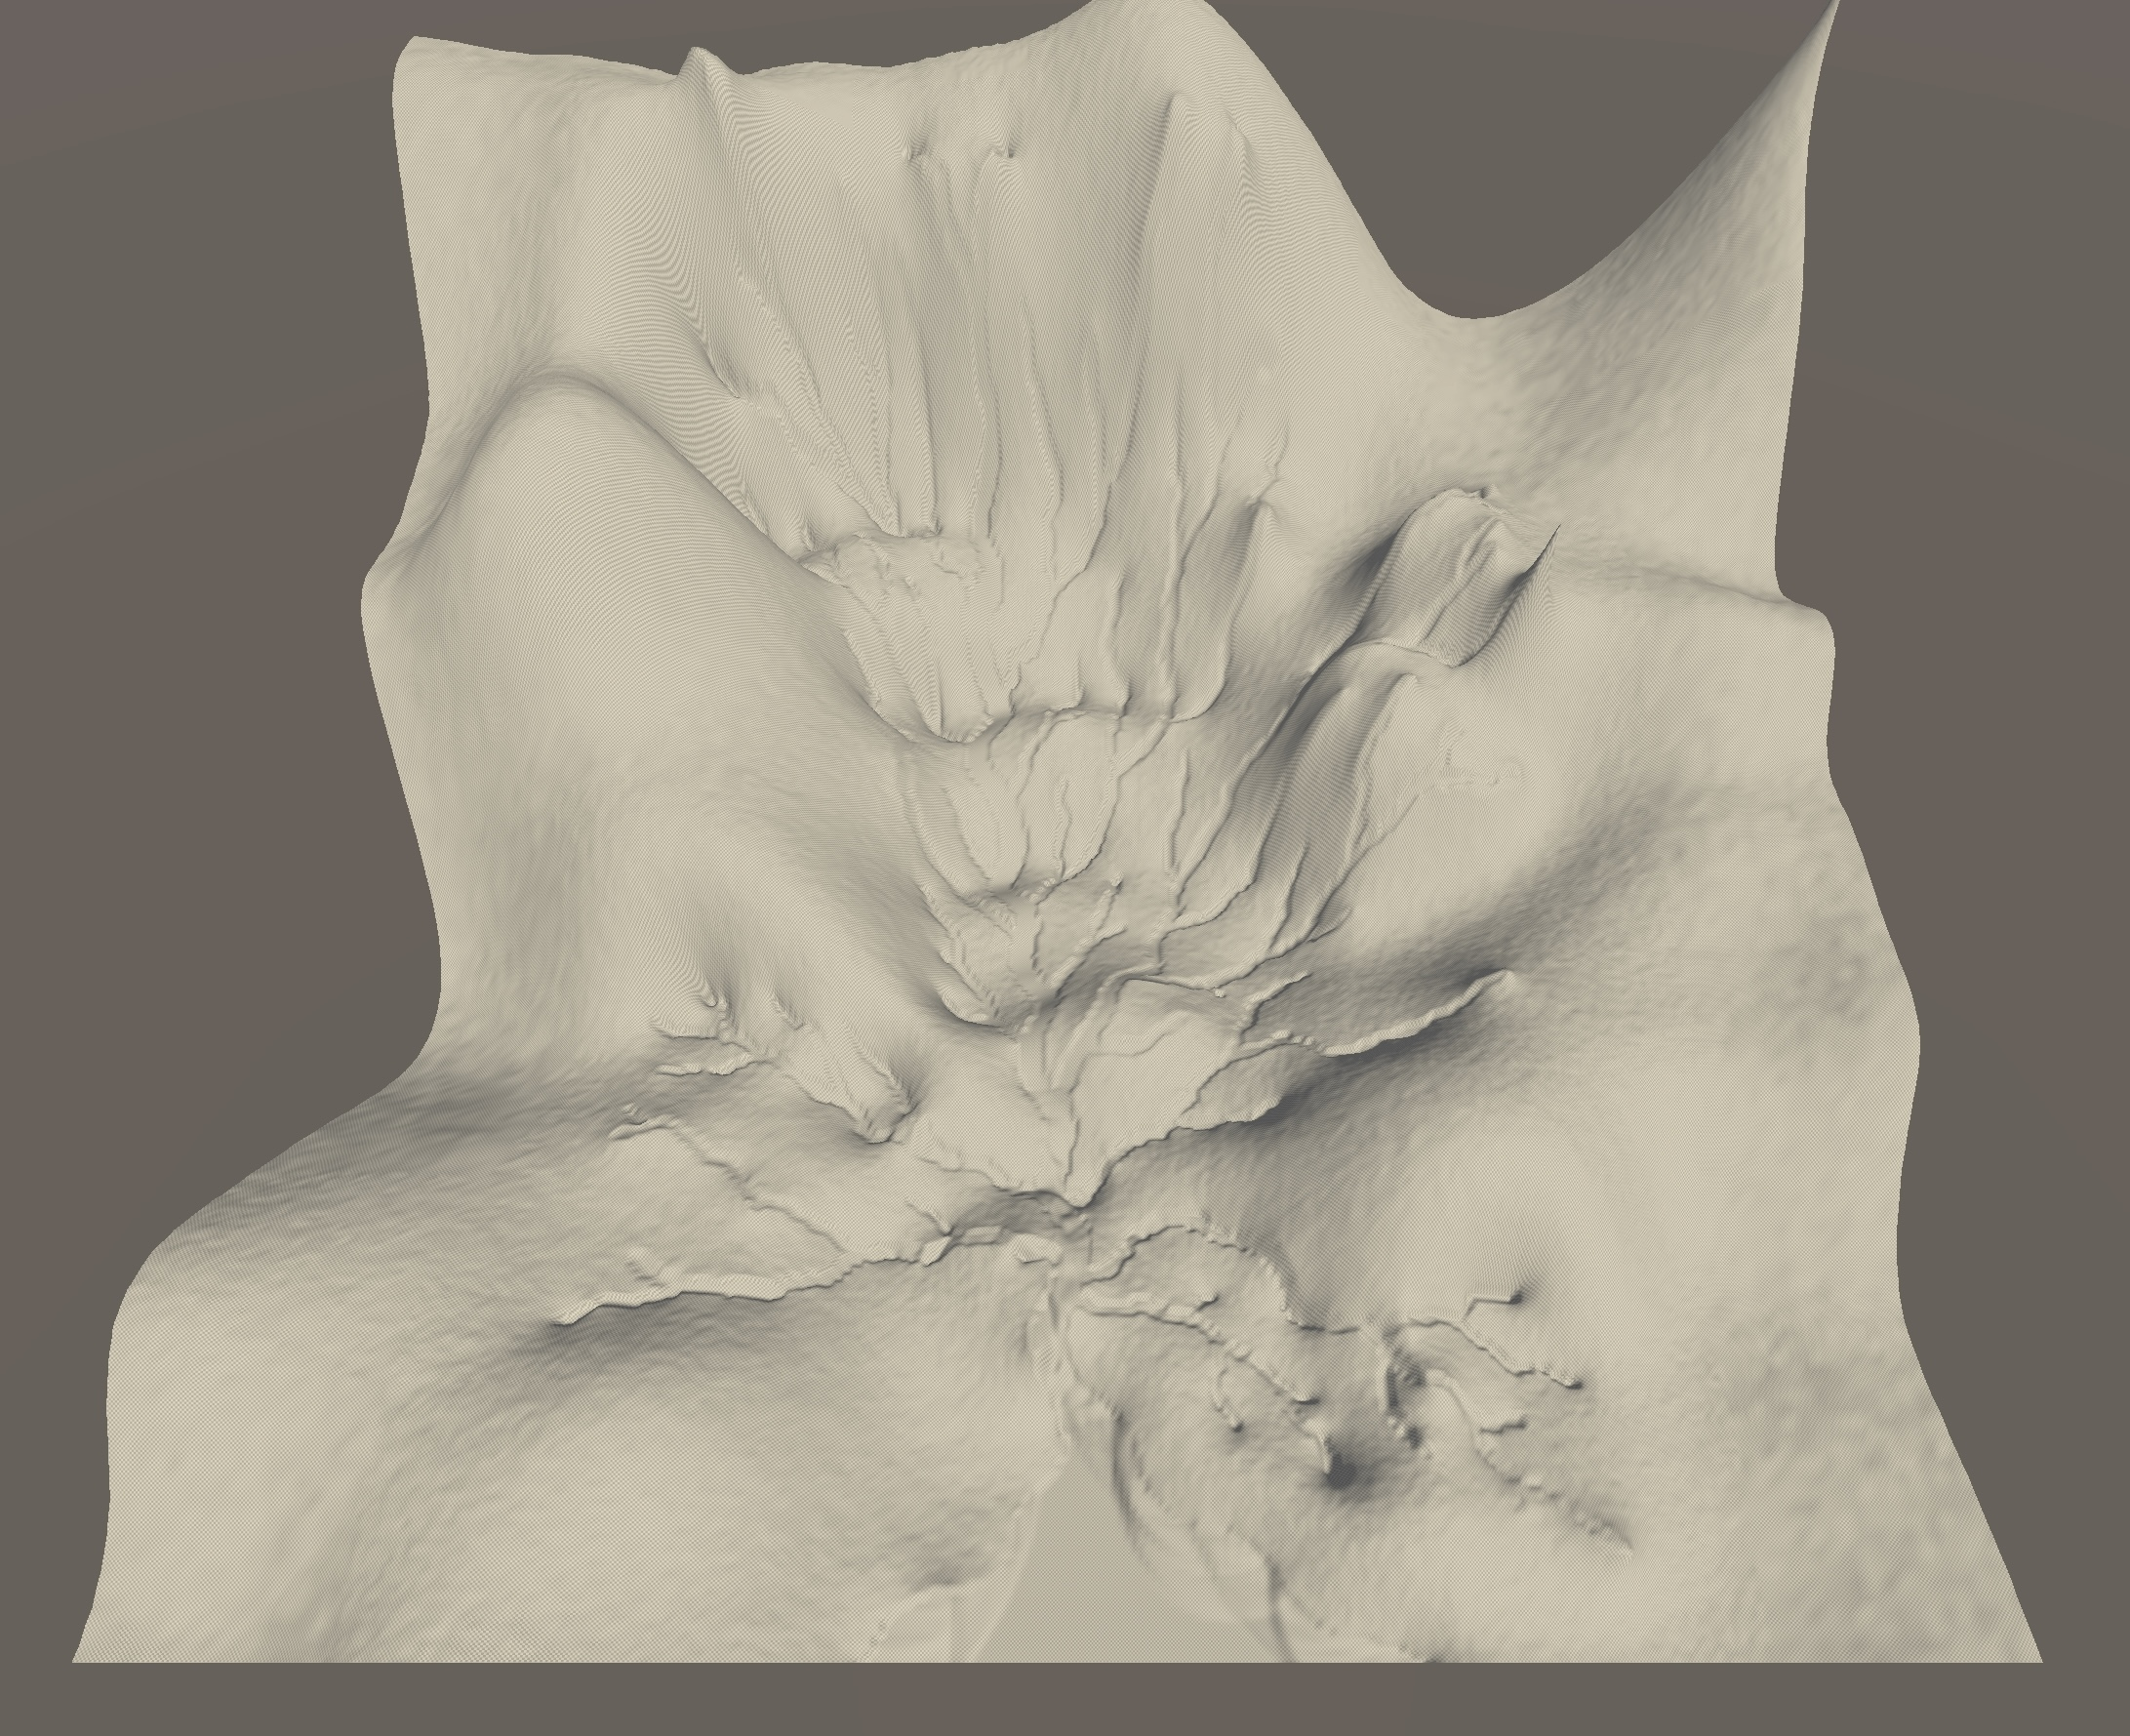
\includegraphics[width=0.5\linewidth]{img/evaluation/3/manual_image_3.jpg}
    \caption{Resulting terrain for \ref{fig:constraint_3} generated using manually set terrain operation.}
    \label{fig:manual_image_3}
\end{figure}

\textbf{IGA Approach:} In Fig. \ref{fig:iga_image_3}, we can see an example of a terrain generated using the IGA approach.

\begin{figure}[h!]
    \centering
    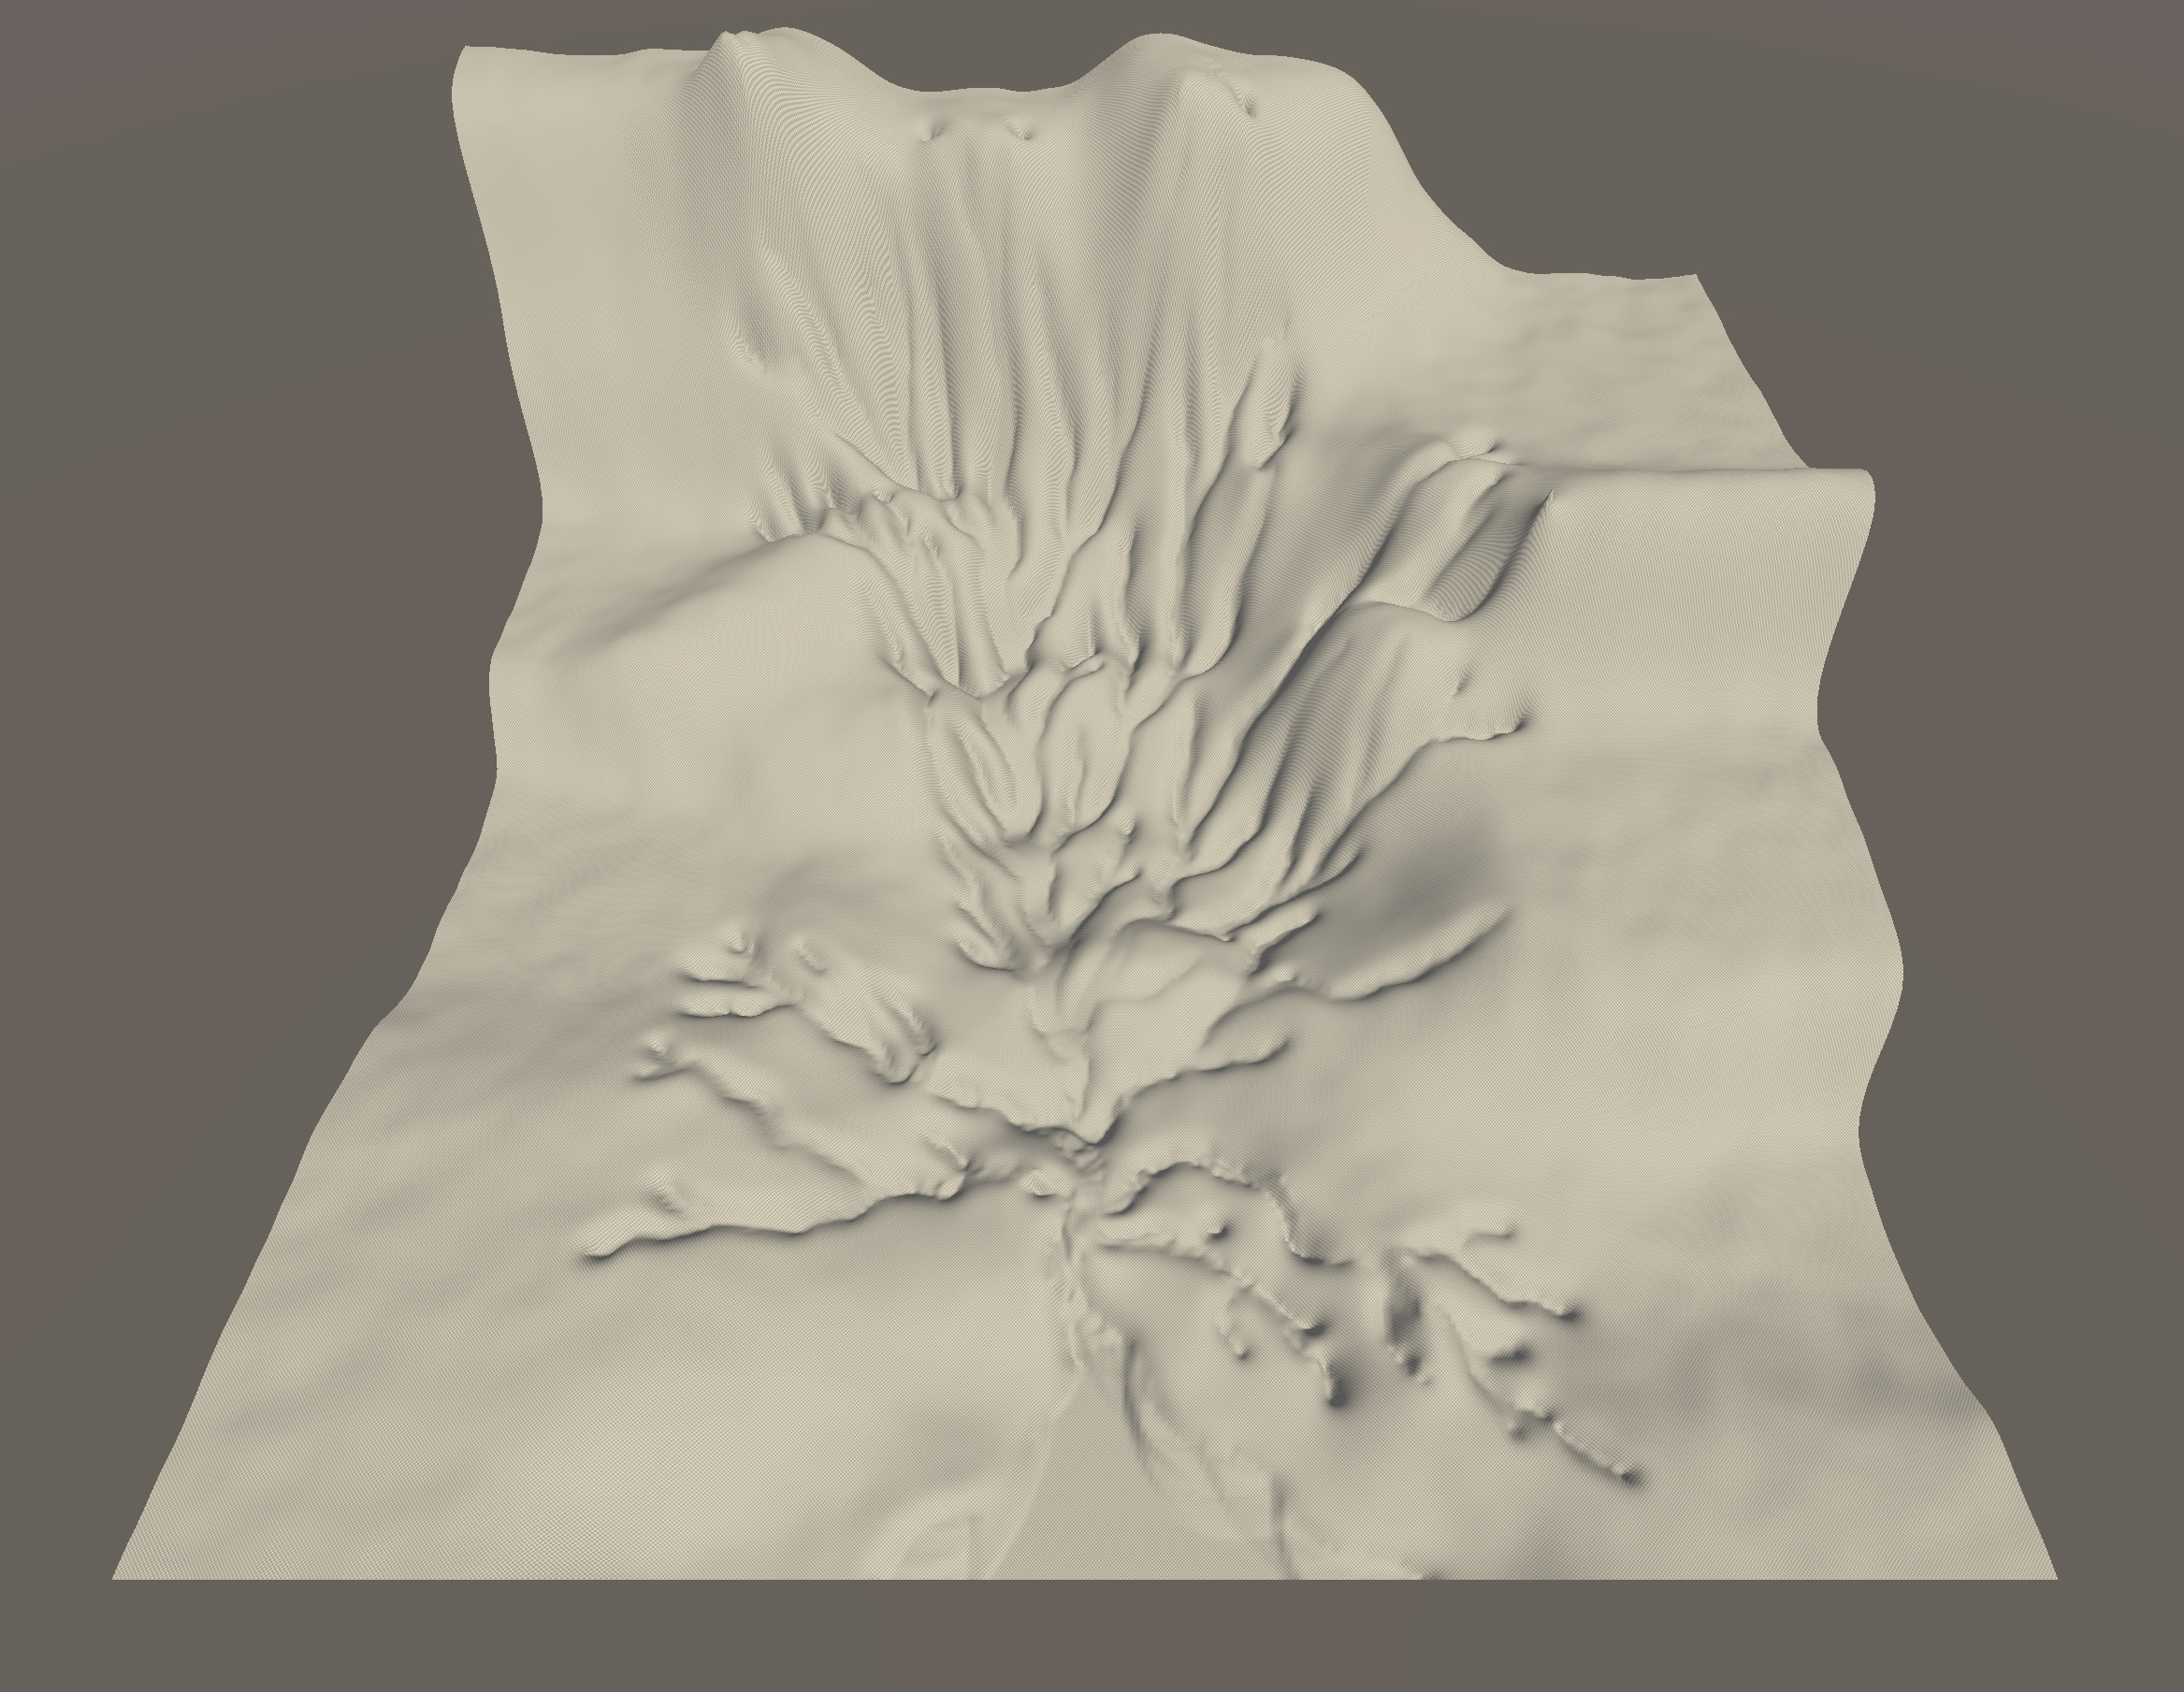
\includegraphics[width=0.5\linewidth]{img/evaluation/3/iga_image_3.jpg}
    \caption{Resulting terrain for \ref{fig:constraint_3} generated using the IGA evolution window.}
    \label{fig:iga_image_3}
\end{figure}


% Case Study 4
\subsection{Island/Coastline network constraint}

This case study aims to show our system's ability to deal with generating the land bordering bodies of water. The constrained area represents flat water, and then we aim to modify the island/land to have natural coastlines, which tend to have smooth transitions into the water.
In our example, we will use the constraint combination as seen in Fig. \ref{fig:constraint_4}:

\begin{figure}[H]
    \centering
    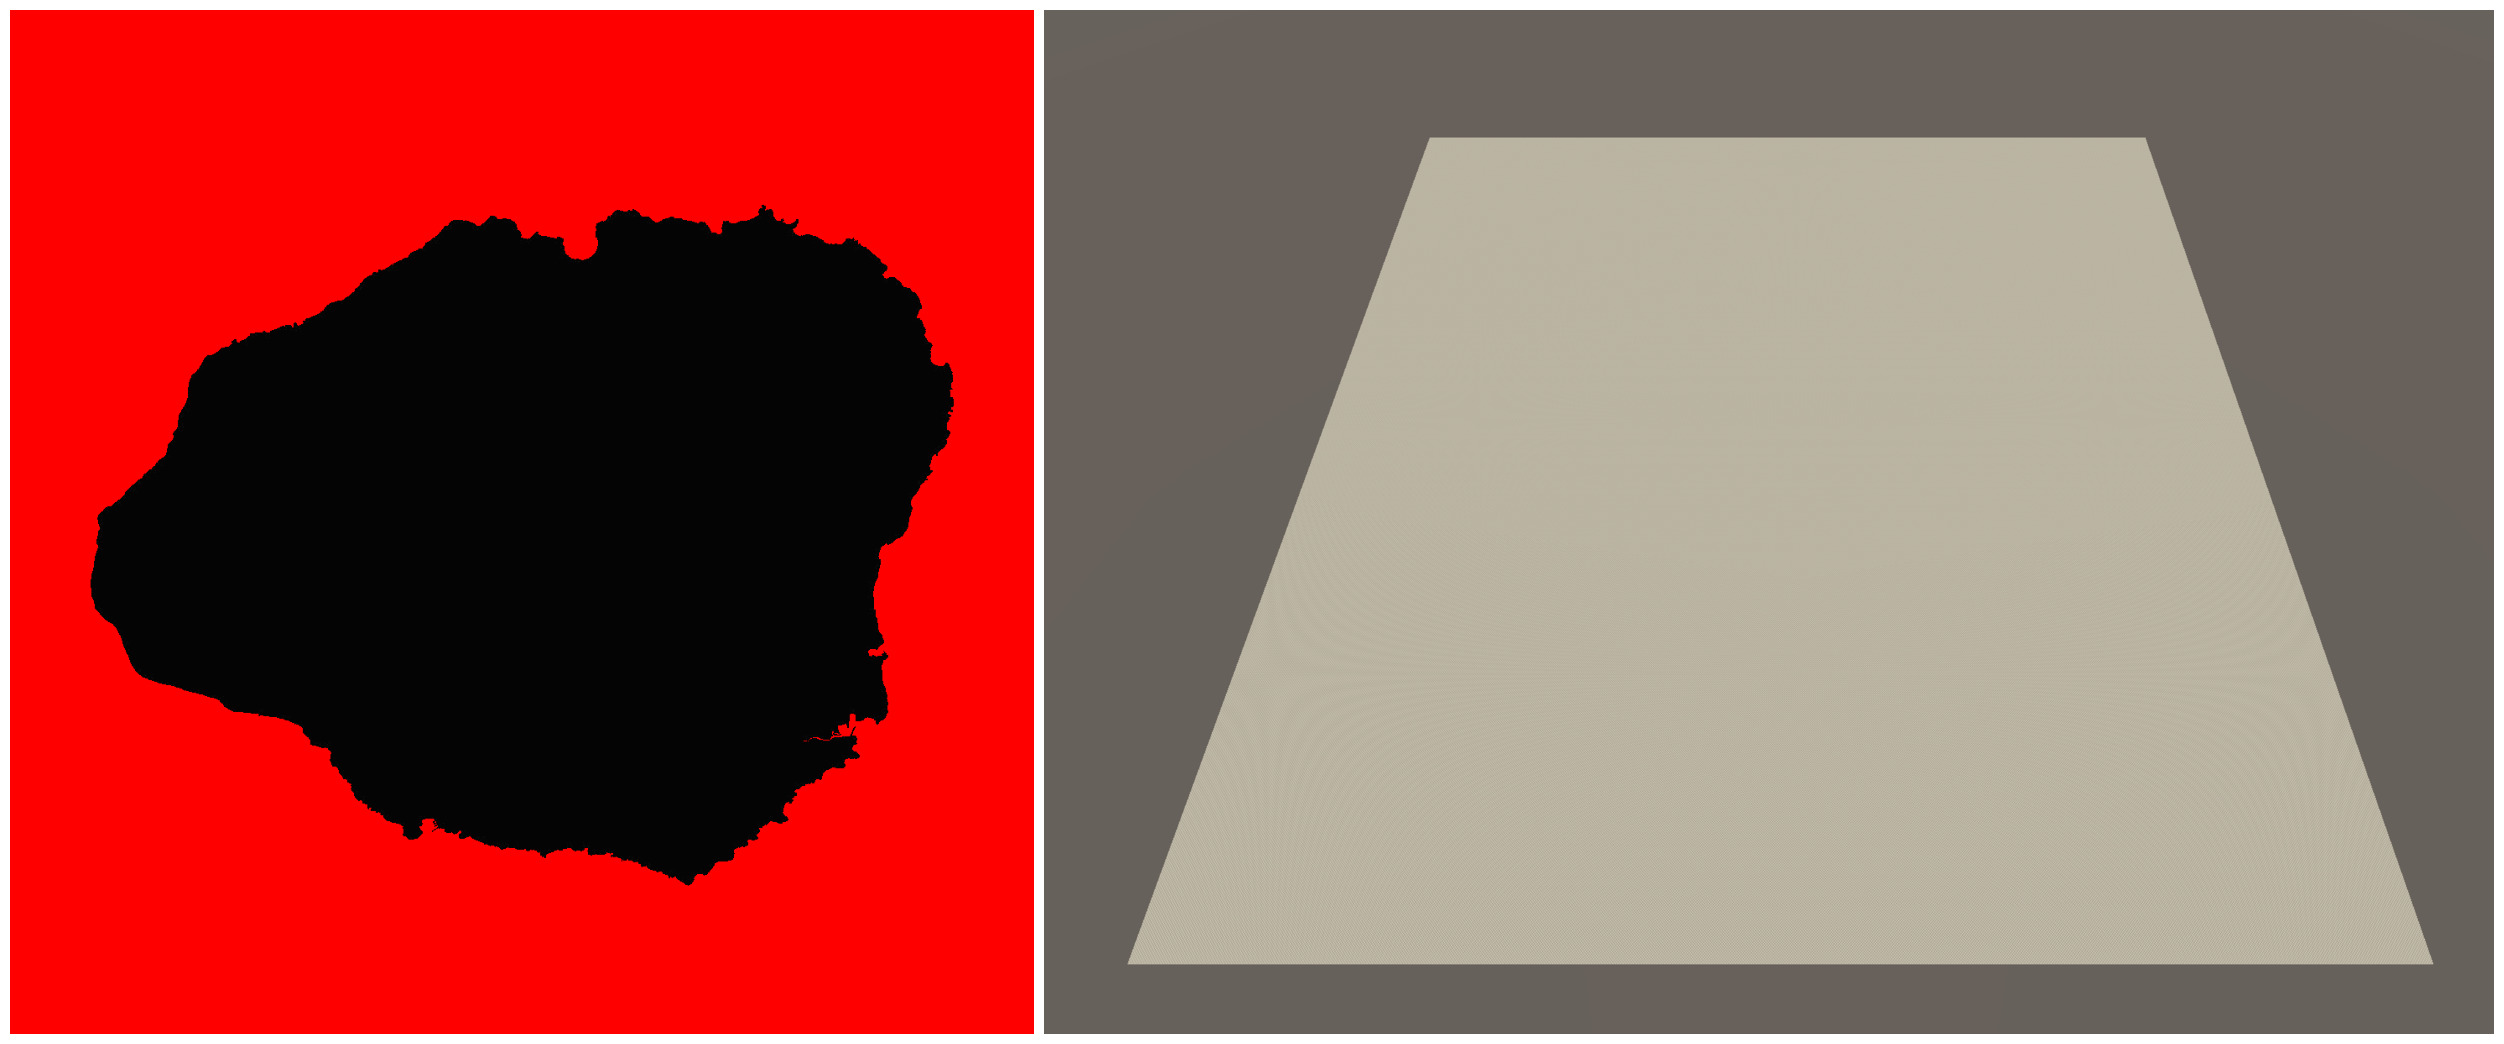
\includegraphics[width=0.5\linewidth]{img/evaluation/4/constraint_4.jpg}
    \caption{The input into our system. (Left) shows the mask texture provided. (Right) shows the set heights for the pixels mapped out by the mask texture. }
    \label{fig:constraint_4}
\end{figure}

\textbf{Manual Approach:} In Fig \ref{fig:manual_image_4}, we can see an example of a terrain generated using the manual interaction approach.

\begin{figure}[H]
    \centering
    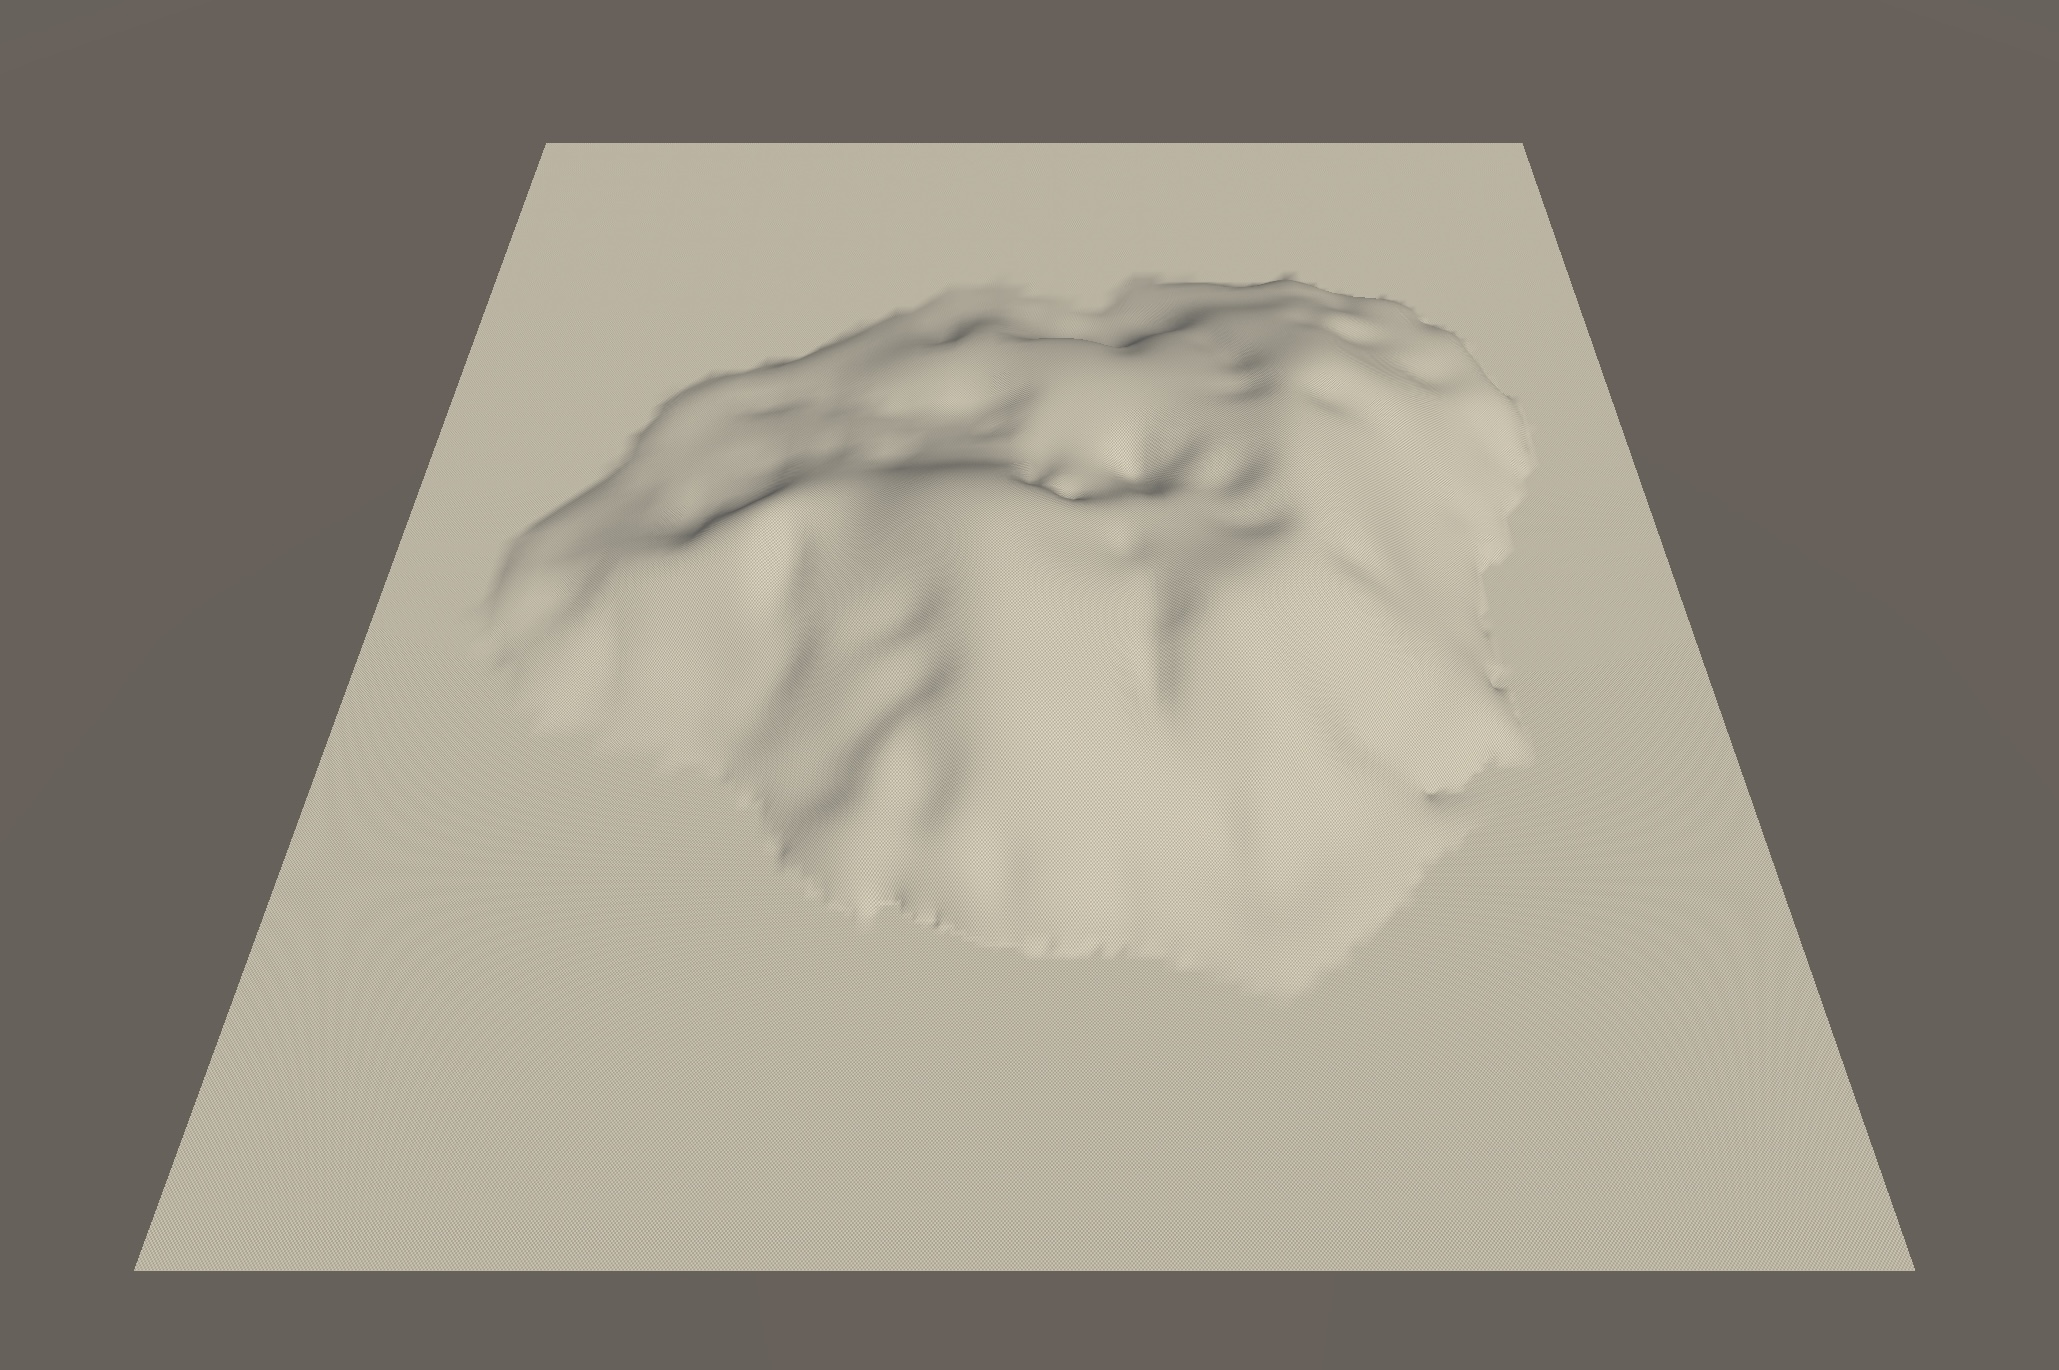
\includegraphics[width=0.5\linewidth]{img/evaluation/4/manual_image_4.jpg}
    \caption{Resulting terrain for \ref{fig:constraint_4} generated using manually set terrain operations.}
    \label{fig:manual_image_4}
\end{figure}

\textbf{IGA Approach:} In Fig. \ref{fig:iga_image_4}, we can see an example of a terrain generated using the IGA approach.

\begin{figure}[H]
    \centering
    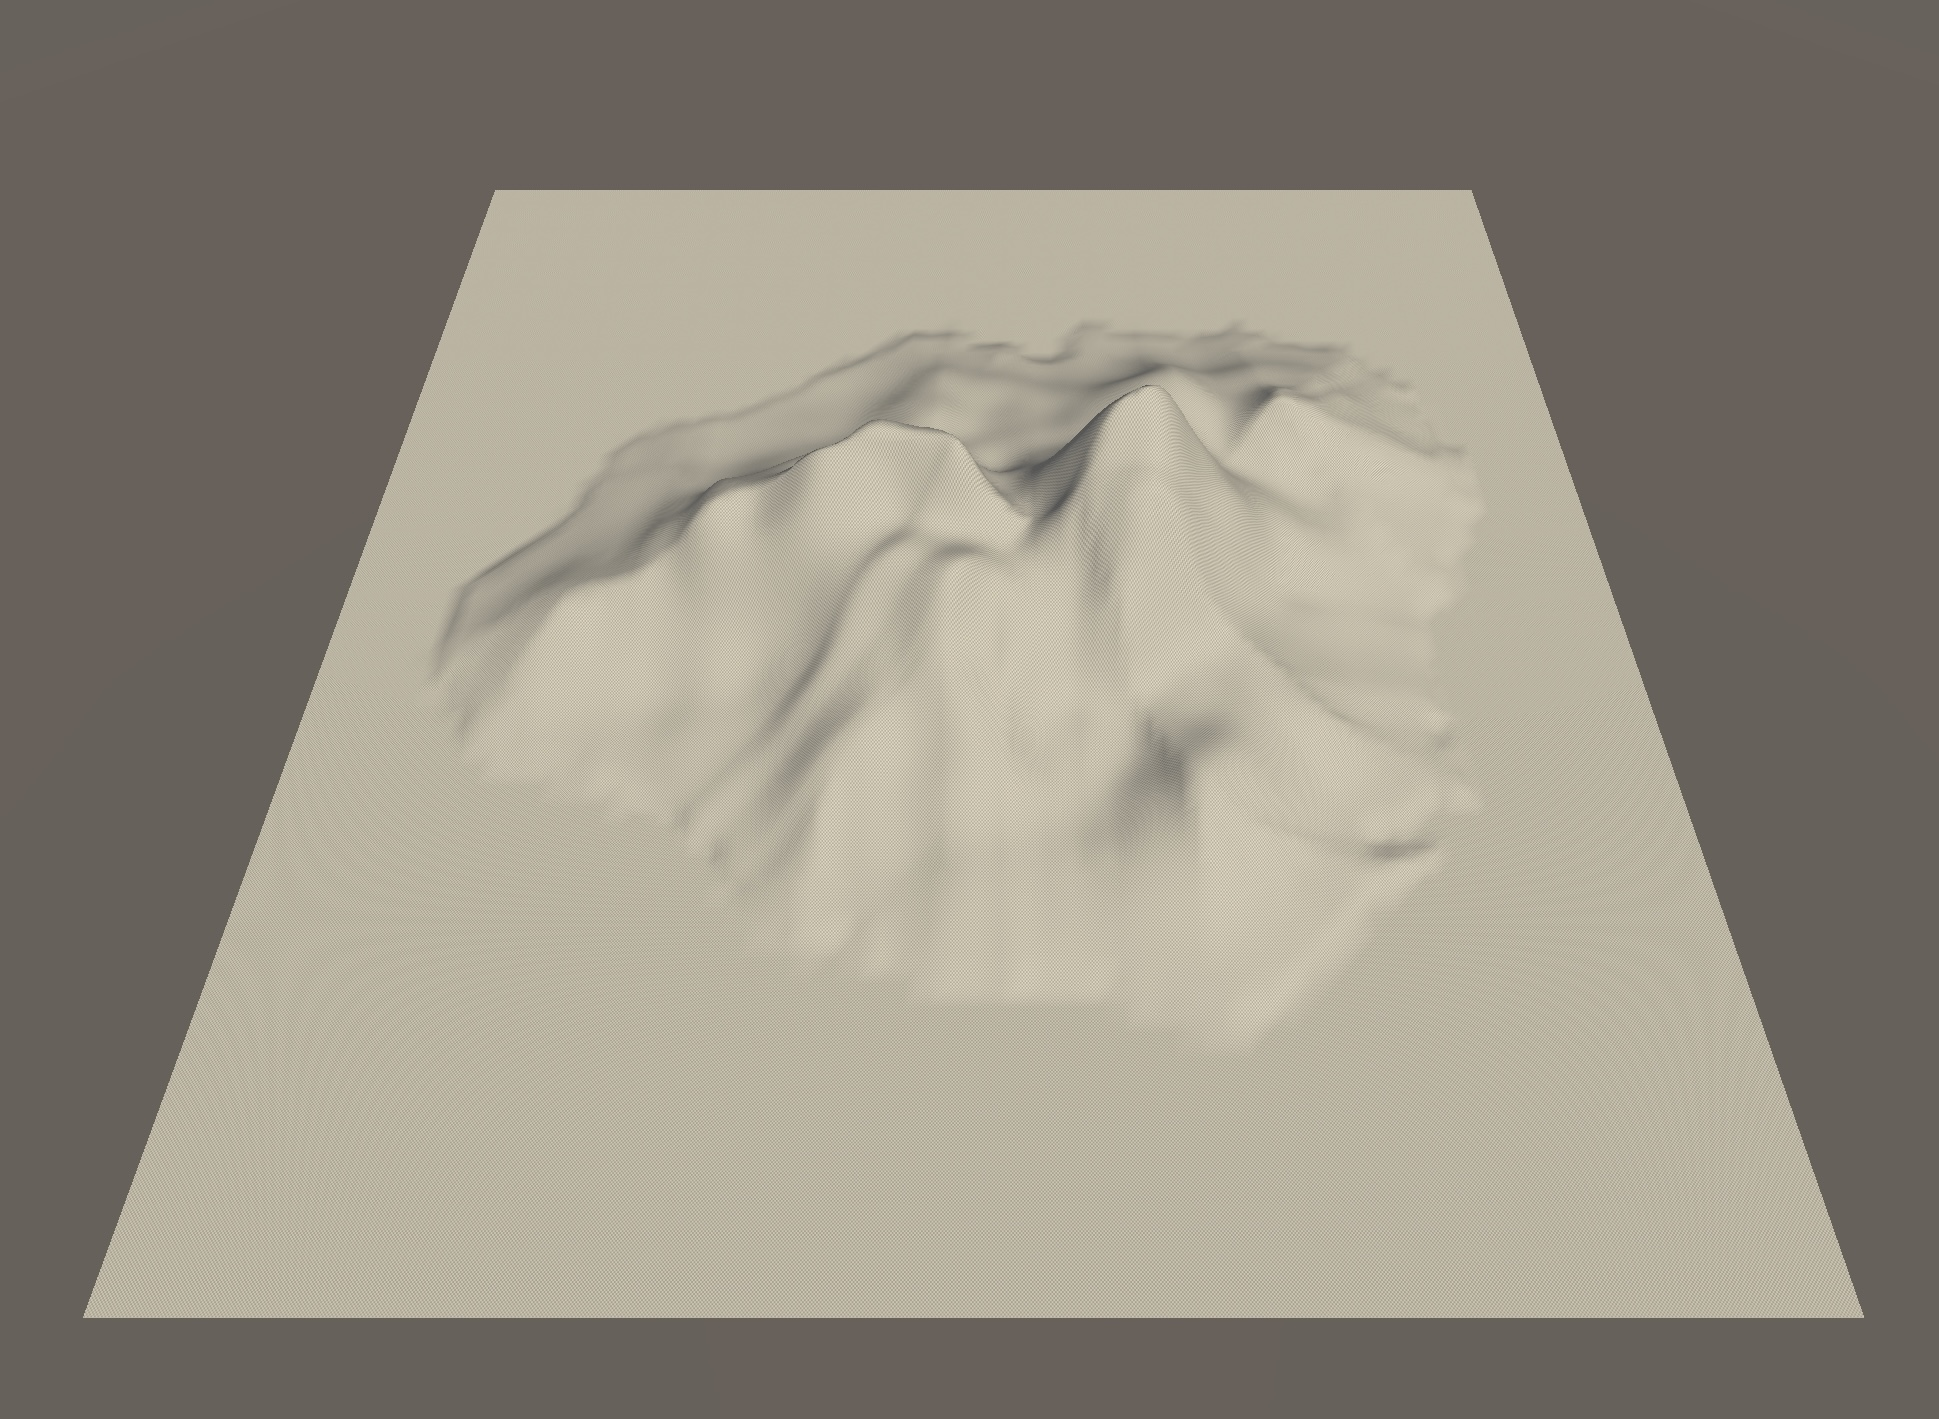
\includegraphics[width=0.55\linewidth]{img/evaluation/4/iga_image_4.jpg}
    \caption{Resulting terrain for \ref{fig:constraint_4} generated using the IGA evolution window.}
    \label{fig:iga_image_4}
\end{figure}

% Case Study 5
\subsection{Combination of man-made and natural features constraint}

This case study aims to show our systems ability to deal with a combination of different use cases in one terrain. Here, we interpret part of the constraint to represent a building foundation, which has connecting roads (both man-made) as well as the other parts to represent a dam and a mountain (natural features). We aim for our system to fill in the heights of the modifiable areas to connect all these constrained areas in a coherent and natural way.

In our example, we will use the constraint combination as seen in Fig. \ref{fig:constraint_5}, with the mask texture seen on the left, and the respective predefined heights seen on the right.

\begin{figure}[H]
    \centering
    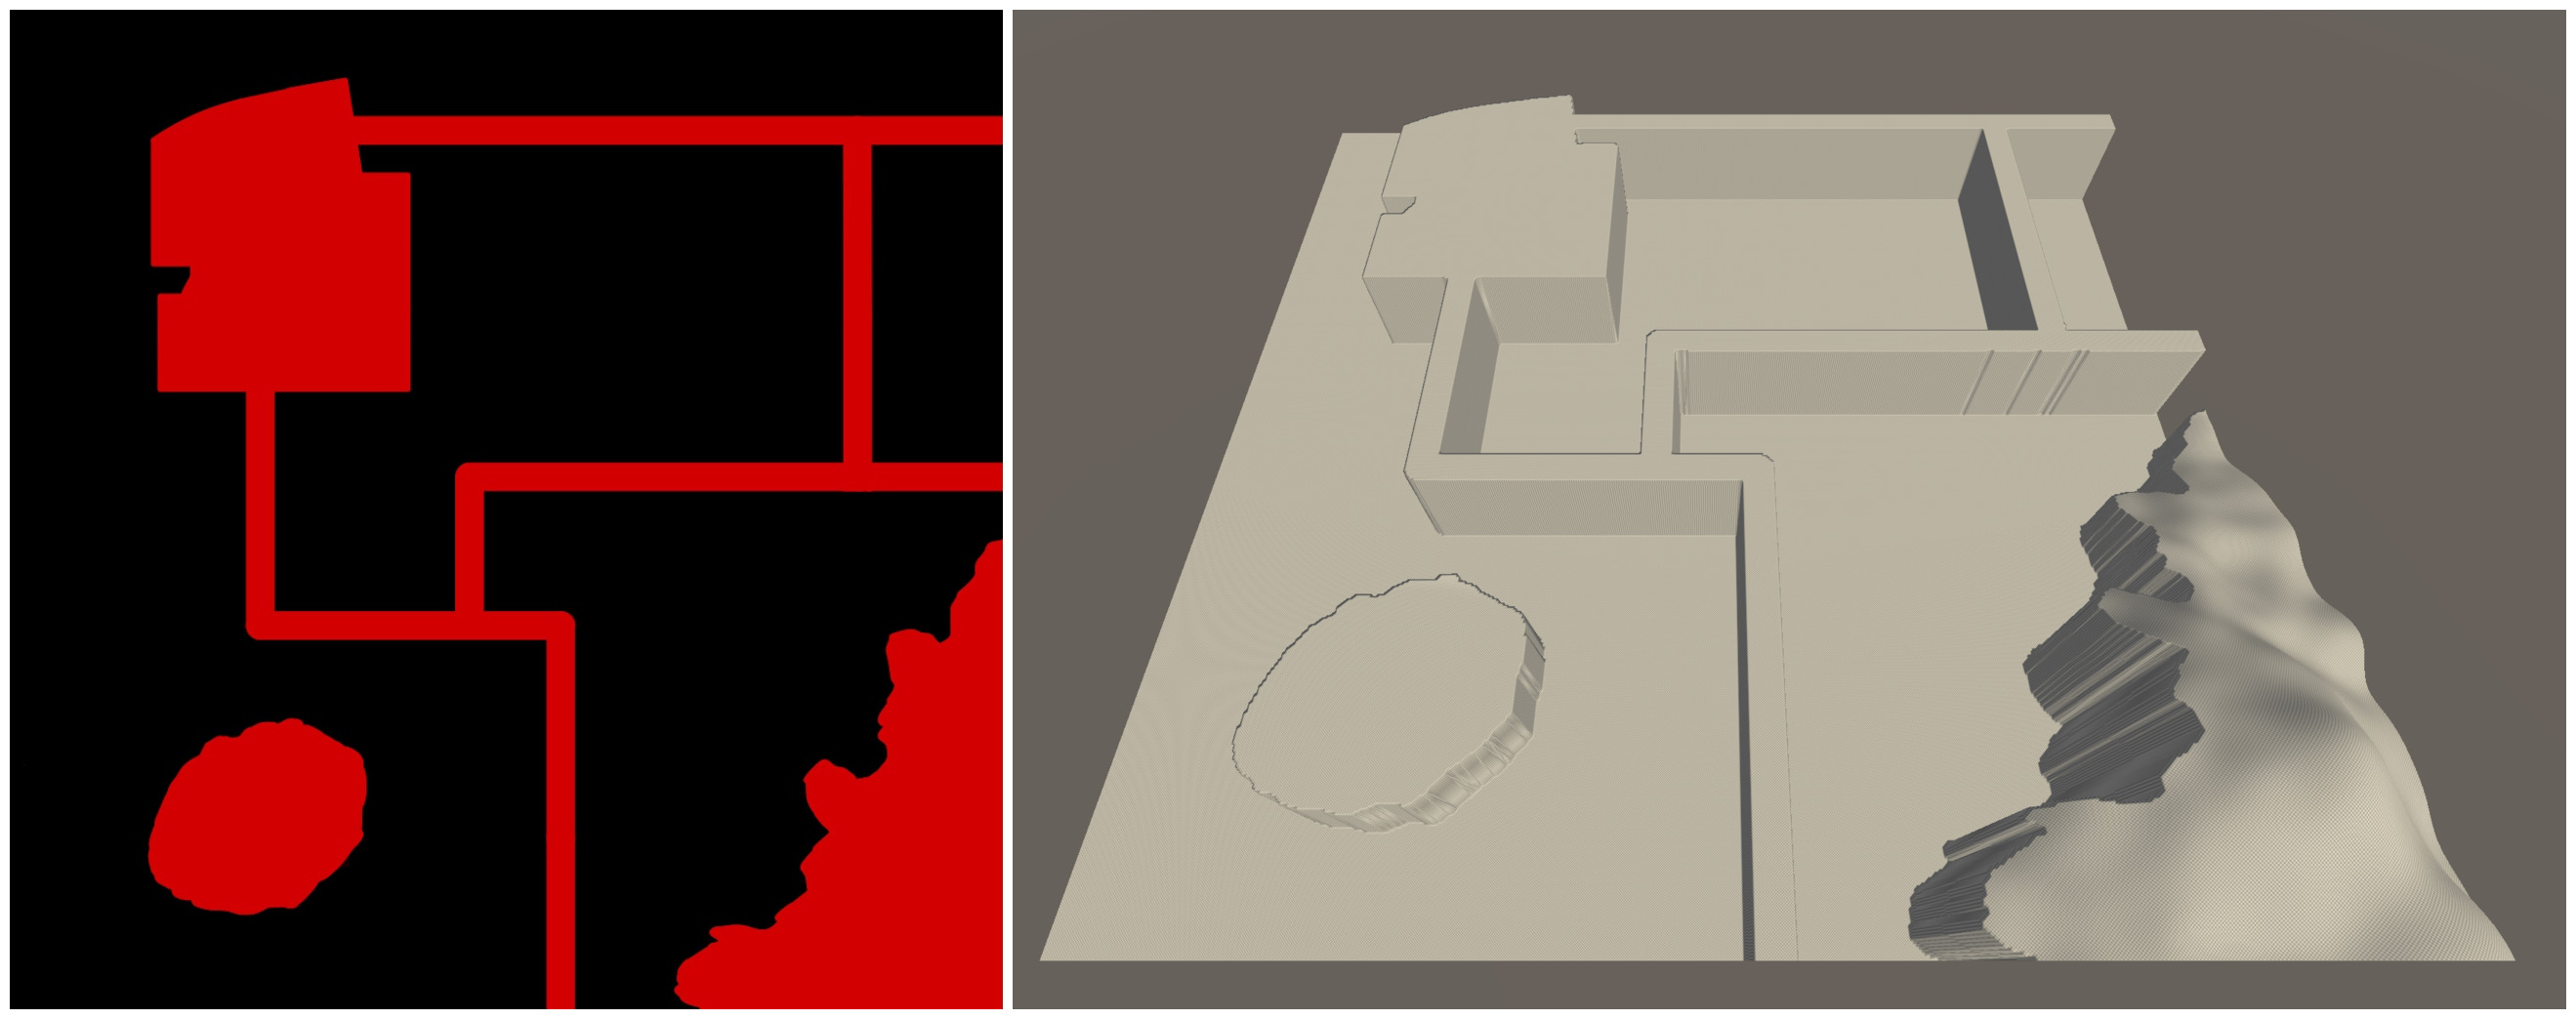
\includegraphics[width=0.75\linewidth]{img/evaluation/5/constraint_5.jpg}
    \caption{The input into our system. (Left) shows the mask texture provided. (Right) shows the set heights for the pixels mapped out by the mask texture.}
    \label{fig:constraint_5}
\end{figure}

\textbf{Manual Approach:} In Fig. \ref{fig:manual_image_5}, we can see an example of a terrain generated using the manual interaction approach.

\begin{figure}[H]
    \centering
    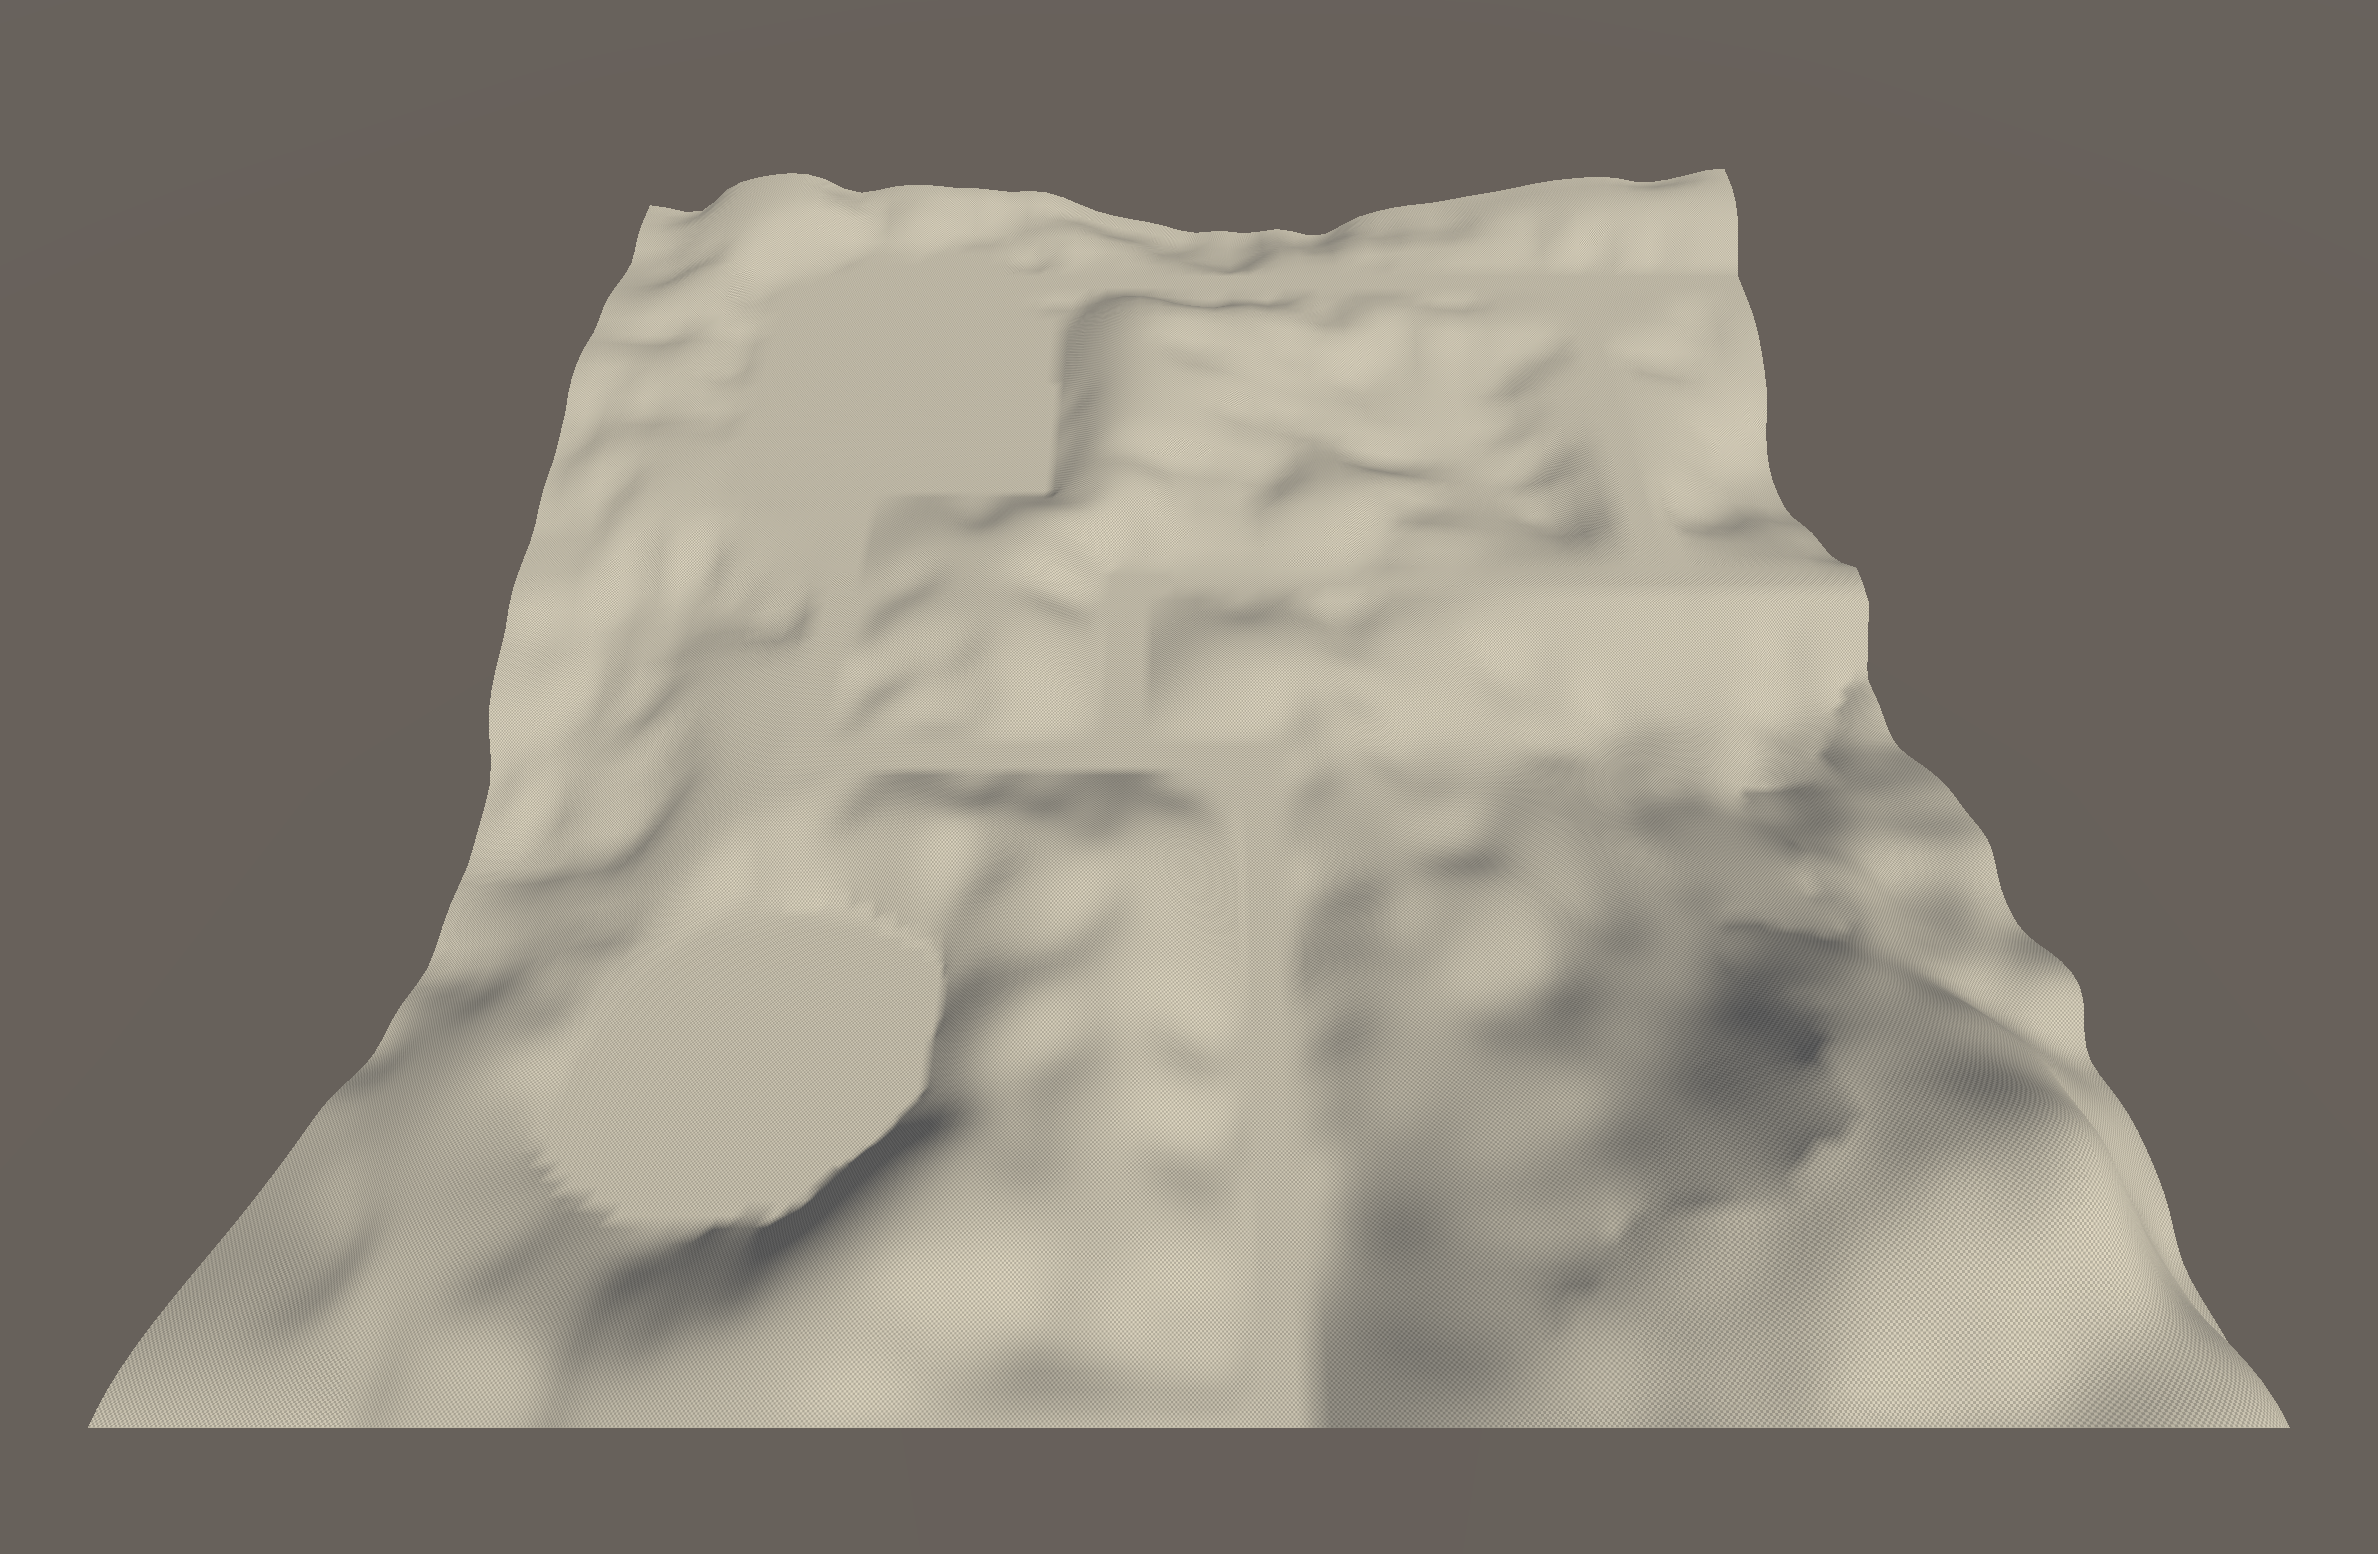
\includegraphics[width=0.55\linewidth]{img/evaluation/5/manual_image_5.png}
    \caption{Resulting terrain for \ref{fig:constraint_5} generated using manually set terrain operations.}
    \label{fig:manual_image_5}
\end{figure}

\textbf{IGA Approach:} In Fig. \ref{fig:iga_image_5}, we can see an example of a terrain generated using the IGA approach.

\begin{figure}[H]
    \centering
    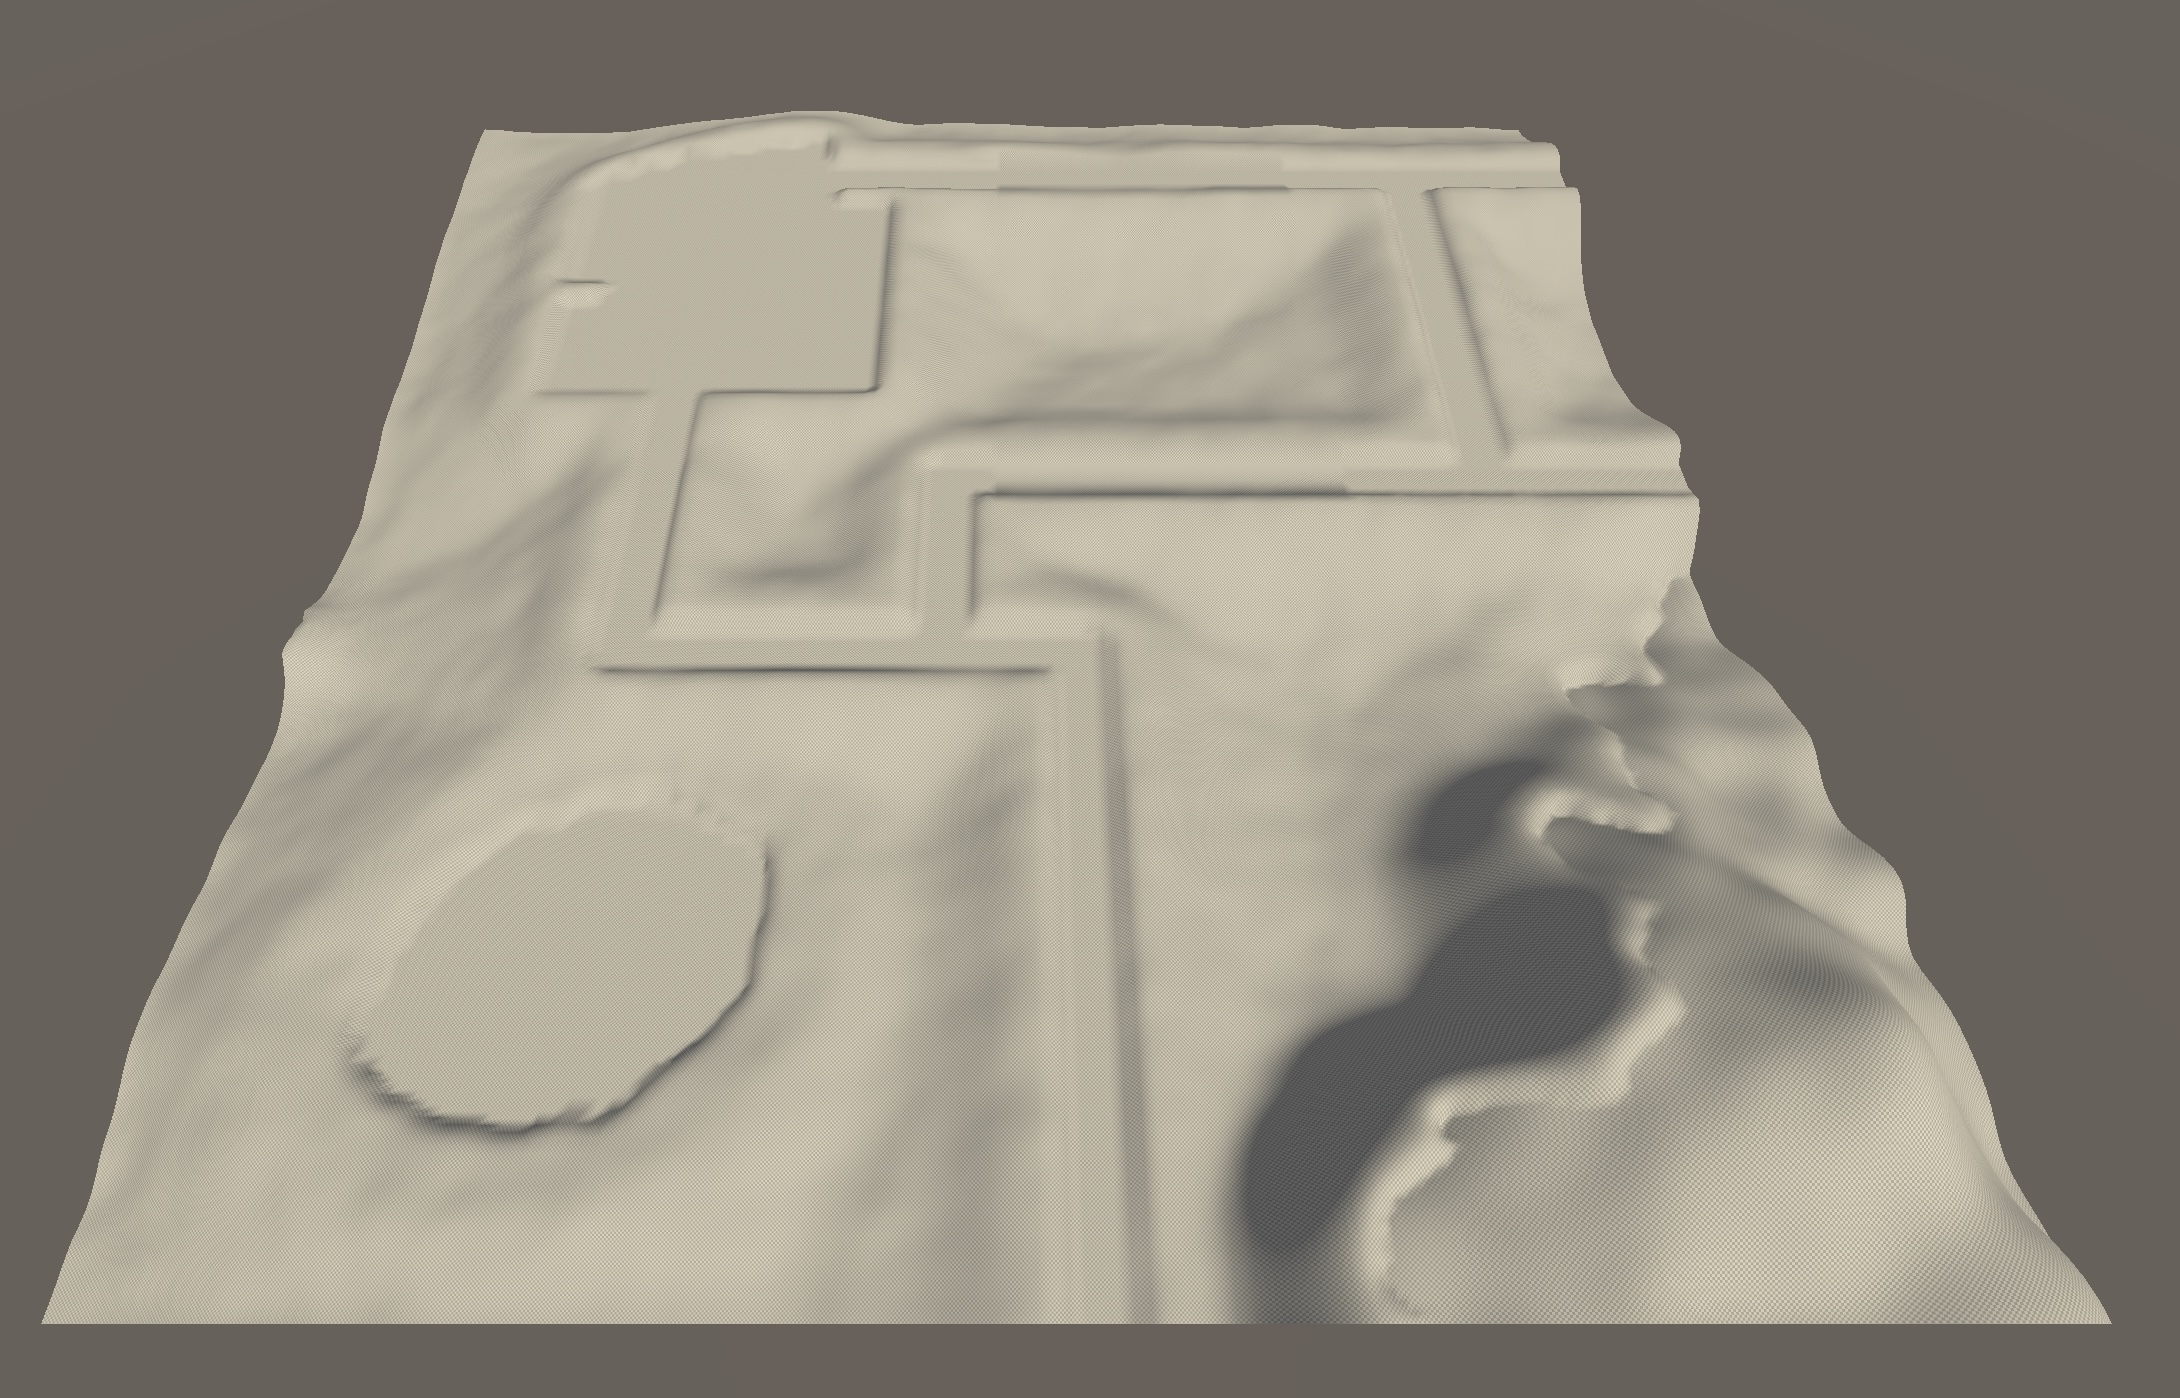
\includegraphics[width=0.55\linewidth]{img/evaluation/5/iga_image_5.jpg}
    \caption{Resulting terrain for \ref{fig:constraint_5} generated using the IGA evolution window.}
    \label{fig:iga_image_5}
\end{figure}


\section{Visual Analysis}

\subsection{Our Own Analysis of Case Studies}

Evaluating our results across the five case studies according to the visual criteria established in Section \ref{visual_crit}, we observe several noteworthy patterns and achievements in our distance-based approach.

\textbf{Smooth Transitions:} Our system demonstrates excellent performance in creating seamless blending between fixed and procedurally generated areas. This is particularly evident in the foundations constraint case study (Figure \ref{fig:manual_image_2}), where the original constraint boundaries become virtually invisible, fully integrated into the surrounding terrain. Across all case studies, we consistently avoid sharp transitions at constraint boundaries, achieving the natural flow that was our primary objective. The most challenging scenario occurred in the combination constraint case study using the IGA approach (Figure \ref{fig:iga_image_5}), where blending into the predefined mountain in the bottom-right corner proved more difficult, though still achieving acceptable integration.

\textbf{Geological Possibility:} Our generated terrains consistently exhibit formations that could feasibly exist in nature. The island/coastline constraint case study (Figures \ref{fig:manual_image_4} and \ref{fig:iga_image_4}) particularly excels in this regard, creating realistic coastal transitions that mirror natural shoreline formations. However, we observe that the river constraint generated using the IGA approach (Figure \ref{fig:iga_image_3}) occasionally exhibits patterns that appear more algorithmically generated, suggesting that our evolutionary approach may require further refinement for certain constraint types.

\textbf{Contextual Coherence:} The road/path network constraint case study (Figures \ref{fig:manual_image_1} and \ref{fig:iga_image_1}) demonstrates exceptional contextual integration, where the road infrastructure appears naturally embedded within the landscape rather than artificially imposed. This success extends to our general handling of linear path constraints, confirming that our distance-based methodology is particularly well-suited for this.

\textbf{Feature Variety:} Our system successfully generates diverse terrain characteristics ranging from smooth, rolling hills to textured, bumpy surfaces, from mountainous regions to flat plains. This variability reflects both the flexibility of our parameter space and the effectiveness of our Interactive Genetic Algorithm in exploring different aesthetic preferences. The diversity demonstrates that our approach adapts well to different user preferences and constraint contexts.

Ranking our case studies by overall visual success, we would order them as follows: (1) road/path network, (2) island/coastline, (3) foundations, (4) river network, and (5) combination constraints. This ranking reflects both the naturalness of results and the complexity of successfully integrating multiple constraint types simultaneously.

\subsection{Comparison with Bottom-Up Methods}

Bottom-up approaches, as exemplified by \cite{Belhadj07} and described in Section \ref{bottom_up_method}, work outward from constraints to generate surrounding terrain. We compare our results from the river network case study (Figures \ref{fig:manual_image_3} and \ref{fig:iga_image_3}) with the results from the bottom-up method shown in Fig. \ref{fig:belhadj_final_result}.

\begin{figure}[H]
    \centering
    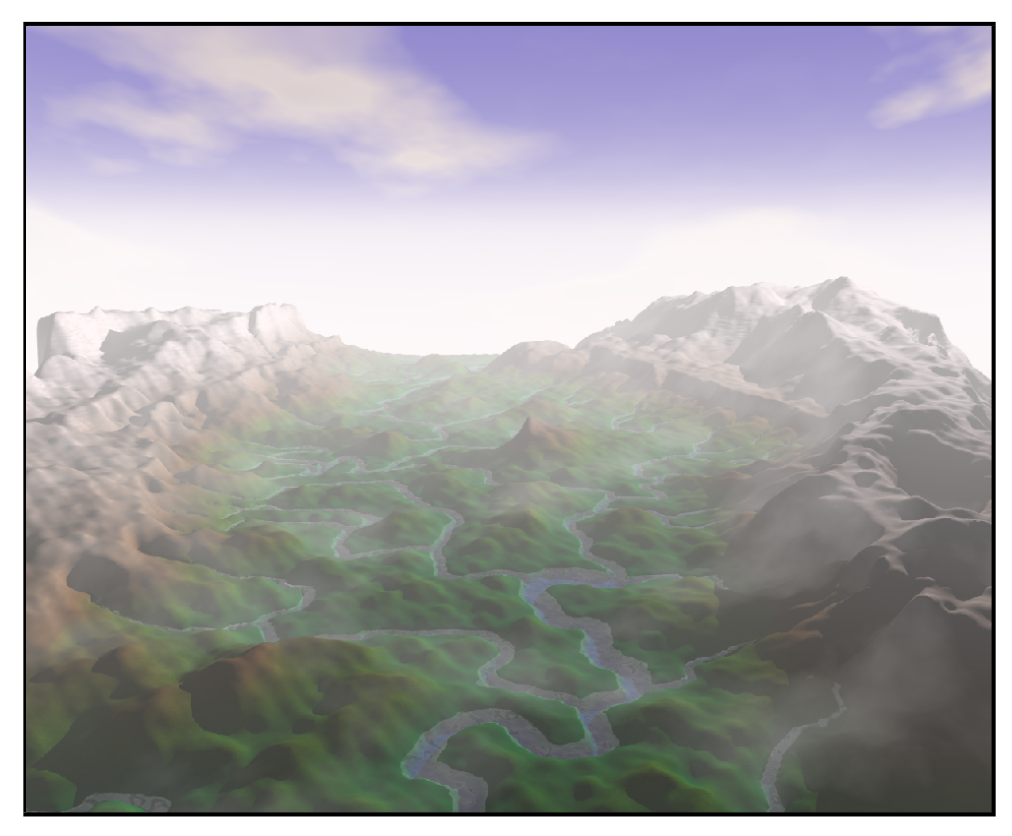
\includegraphics[width=0.6\textwidth]{img/previous_works/belhadj_result.png}
    \caption{Final terrain model generated using a two-step interpolation process (MDI followed by MD), showing smooth integration between fixed ridge and river networks and the surrounding terrain. Source: \cite{Belhadj07}.}
    \label{fig:belhadj_final_result}
\end{figure}

We acknowledge that their method produces highly natural results for river networks, scoring well according to our visual criteria. Their transitions are exceptionally gentle into the river constraints with no noticeable artifacts, demonstrating the effectiveness of their specialised approach for this specific constraint type.

However, our approach demonstrates superior handling of scenarios with \textbf{large height disparities}. While their work does not extensively demonstrate performance with significant elevation differences, our system successfully manages such challenging constraints, as evidenced in our \textit{river network case study} where substantial height variations exist between source and destination points of the river. This capability represents a significant advantage for real-world applications where terrain constraints often involve \textbf{dramatic elevation changes}.

Regarding surrounding terrain quality, we observe that the bottom-up approach, which relies primarily on midpoint displacement and inverse displacement interpolation, lacks the sophisticated \textbf{erosion} and \textbf{detail enhancement} features present in our system. Consequently, while their constraint integration is excellent, the surrounding terrain exhibits less natural variation and detail compared to our results. Our manual approach achieves naturalness levels closely comparable to their specialised method, while our IGA approach, though not quite matching their quality, still produces acceptable results for this constraint type.

\subsection{Comparison with Path-based Constraint Methods}

The path-based terrain generation approach developed by \cite{Andereck14}, shown in Figure \ref{fig:andereck_path}, presents an interesting alternative methodology for handling linear constraints. We compare this with our path/road constraint in Figure \ref{fig:manual_image_1} and Figure \ref{fig:iga_image_1}. 

\begin{figure}[h!]
    \centering
    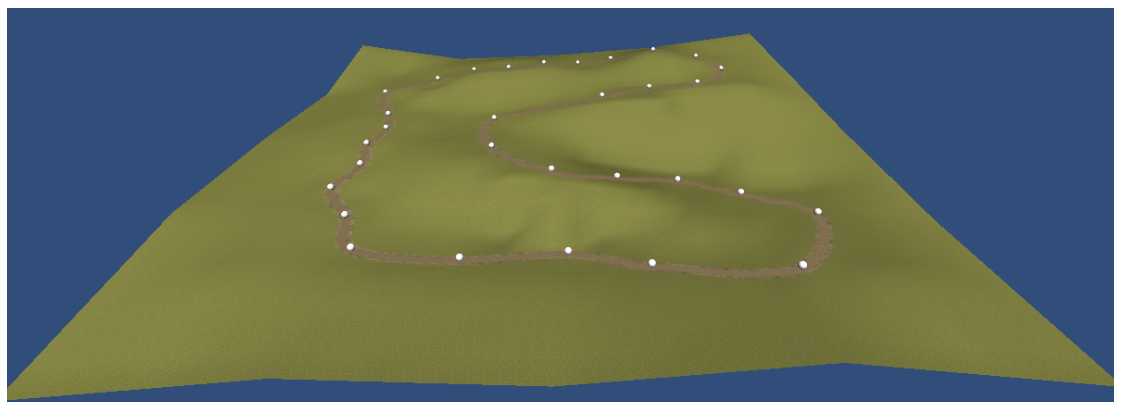
\includegraphics[width=0.6\textwidth]{img/previous_works/adereck_path_result.png}
    \caption{Path-based terrain generation that preserves the exact heights of pre-defined paths while procedurally generating surrounding terrain features. Source: \cite{Andereck14}.}
    \label{fig:andereck_path}
\end{figure}

While their approach demonstrates good transitions and overall natural appearance around the path constraints, we believe our method provides superior results in several key areas. Most notably, our surrounding terrain exhibits significantly greater \textbf{diversity} and \textbf{naturalness}. Their method appears to focus primarily on creating relatively flat terrains around paths that blend smoothly but lack the rich variation and \textit{realistic geological features} that our system produces.

Additionally, our system can adapt to various constraint types beyond just paths, whereas their approach is more specifically tailored to linear path constraints. Even for path-based constraints only, we consider our system to provide a more comprehensive and flexible solution.

\subsection{Manual vs IGA Parameter Tuning}

The comparison between manual parameter adjustment and our Interactive Genetic Algorithm approach reveals important insights about both approaches' capabilities and limitations.

The most significant quality difference between manual and IGA approaches appears in the \textit{river network constraint case study}, where the manual approach (Figure \ref{fig:manual_image_3}) produces more natural-looking terrain compared to the IGA result (Figure \ref{fig:iga_image_3}). This difference highlights that when dealing with complex constraint types requiring nuanced parameter combinations, expert manual tuning can achieve superior results.

However, our evaluation reveals cases where the IGA approach produces preferred results. Notably, in the \textit{island/coastline case study} (Figure \ref{fig:iga_image_4}), we consider the IGA-generated terrain to look better than the manual approach (Figure \ref{fig:manual_image_4}), demonstrating the algorithm's ability to discover unexpected but aesthetically pleasing parameter combinations.

The terrain differences between manual and IGA approaches often reflect genuine variations in aesthetic preference rather than quality deficiencies. The IGA's goal is not to mimic manual expert tuning but to explore the parameter space according to user aesthetic preferences, potentially discovering solutions that manual approaches might not consider.

Manual parameter tuning demonstrates particular advantages when handling constraints with large height disparities. Our IGA system, designed to handle diverse constraint types effectively, prioritises robustness across many normal cases. This design choice means it may struggle with highly specialised scenarios that benefit from expert domain knowledge and targeted parameter selection.

Importantly, both approaches consistently produce results that meet the visual criteria established in Section \ref{visual_crit}. While manual tuning by experts may yield marginally better results in some complex scenarios, the IGA approach successfully democratises the system, enabling non-expert users to achieve satisfactory terrain generation results without requiring deep understanding of the underlying algorithms and parameters.

\section{Performance Evaluation}
\label{performance_eval}

Beyond visual quality assessment, we evaluated the computational performance of our system to understand its practical usability within the Unity development environment. All performance tests were conducted on terrain with a resolution of 1024×1024 heightmap points. Most terrain operations in our system execute with near-instantaneous performance, completing in less than one second. However, certain computationally intensive operations require more detailed performance analysis, which we present in this section.

\subsection{GPU Acceleration Impact}

Our implementation of GPU-accelerated terrain operations demonstrates significant performance improvements over CPU-based alternatives. We evaluated the three primary operations that benefit from GPU acceleration: Basic Smoothing, Enhanced Distance-Based Smoothing, and Thermal Erosion. Each operation was tested using 100 iterations to amplify timing differences and provide measurable performance metrics.

\textbf{GPU Performance:} When utilising compute shader acceleration, all three operations complete their 100-iteration processing in less than one second, demonstrating the substantial computational power available through parallel GPU processing.

\textbf{CPU Performance Comparison:} The CPU fallback implementations, while maintaining algorithmic correctness, exhibit significantly longer processing times:

\begin{itemize}
    \item \textbf{Basic Smoother:} 13 seconds for 100 iterations;
    \item \textbf{Enhanced Distance-Based Smoothing:} 15 seconds for 100 iterations;  
    \item \textbf{Thermal Erosion:} 45 seconds for 100 iterations.
\end{itemize}

The performance difference between GPU and CPU implementations ranges from approximately 13× to over 45× improvement, with thermal erosion showing the most dramatic acceleration. This substantial performance gain demonstrates the effectiveness of our GPU acceleration strategy and justifies the additional implementation complexity.

\textbf{Explaining Performance Differences:} The variation in CPU processing times between operations reflects their computational complexity differences. Basic smoothing performs straightforward neighbourhood averaging, requiring minimal computational overhead per point. Enhanced distance-based smoothing adds distance-aware weight calculations and proximity considerations, resulting in slightly increased processing time.

Thermal erosion exhibits the longest processing time due to its sophisticated material transfer simulation. Unlike simple averaging operations, thermal erosion requires complex neighbour analysis, height difference calculations, and iterative material movement between terrain points. 

\subsection{Interactive Genetic Algorithm Generation Times}

The Interactive Genetic Algorithm component introduces unique performance considerations due to its preview generation requirements. Each terrain genome requires visual preview generation to enable user selection, creating a multiplicative time factor based on population size.

\textbf{Preview Generation Performance:} Individual preview generation averages approximately 5 seconds per genome, with variation ranging from 3 to 8 seconds depending on genome complexity. This variability primarily stems from the number of terrain operations contained within each genome. 

\textbf{Population Size Impact:} The total time required for generating a complete population of terrain previews scales linearly with population size:

\begin{itemize}
    \item \textbf{Population of 8:} Approximately 40 seconds (8 × 5 seconds average)
    \item \textbf{Population of 16:} Approximately 80 seconds (16 × 5 seconds average)  
    \item \textbf{Population of 32:} Approximately 160 seconds (32 × 5 seconds average)
\end{itemize}

While these generation times may initially appear substantial, we consider them acceptable within the context of the IGA's purpose. The Interactive Genetic Algorithm serves to democratise complex terrain generation, enabling non-expert users to achieve sophisticated results without requiring detailed parameter knowledge.

Furthermore, the IGA provides substantial value by exploring parameter combinations that manual approaches might never discover. Users typically require only one high-quality terrain for their specific use case, and once generated, this terrain remains available throughout the development process without requiring regeneration.

The performance characteristics demonstrate that while our Interactive Genetic Algorithm requires meaningful time investment, it provides proportional value through sophisticated parameter exploration and democratised access to complex terrain generation capabilities. For users seeking immediate results, the manual parameter approach remains available with near-instantaneous operation execution.


\section{Summary of Evaluation Results}

Our evaluation across five diverse case studies reveals several key patterns in our system's performance. The distance-based approach consistently excels at creating smooth transitions between fixed and generated terrain, with linear constraints (roads, paths) showing the strongest visual results, while more complex scenarios involving significant height disparities present greater challenges, that our system still overcome. 

The performance analysis reveals a clear trade-off between computational approaches: GPU acceleration provides dramatic speed improvements for intensive operations, while the Interactive Genetic Algorithm introduces longer generation times that are offset by its accessibility to non-expert users. These findings highlight the effectiveness of our hybrid approach, combining rapid individual operations with more time-intensive but intuitive parameter exploration capabilities.




















